\documentclass{report}
\usepackage[a4paper, total={6in, 8in}]{geometry}
\usepackage[toc,page]{appendix}
\usepackage{graphicx}
\usepackage{titling}
\usepackage{array}
\usepackage{lipsum}
\usepackage{booktabs}
\usepackage{appendix}
\usepackage{float}
\usepackage{multirow}
\usepackage{makeidx}
\usepackage[font=small,labelfont=bf]{caption}
\makeindex
\title {
	\includegraphics[width=200pt]{img/"Maynooth University Logo Black RGB 300dpi".png}~\\[1cm]
    {\textbf{Conclave: Making Bitcoin Scale And Be Useful}}
    \newline
    {\small{Final year Project, B.Sc. Honours in Computer Science and Software Engineering}}
    \newline
    {\small{Supervisor: Dr. Phil Maguire }}
}
\date{April 2020}
\author{N. P. O'Donnell, ********}
\begin{document}

\maketitle
\begin{abstract}
A trustless, permissionless, decentralized payment network built atop Bitcoin's base blockchain which allows near-instant, near-feeless payments, including payments to and from the base chain, even if the payee is offline. Deposited funds are locked in multisignature transactions on the base chain whilst users transact on a secondary protocol which stores data on a fast, distributed blockchain. When a user wants to withdraw money back to the base chain, a consensus algorithm ensures the right participants sign the withdrawal. Participants are rewarded with points for withdrawals they sign, and points take a long time to build up. Any participant caught behaving dishonestly loses all their points and has to start again. Collected fees are regularly distributed to participants in proportion to their points.
\end{abstract}
\section*{Declaration}
I hereby certify that this material, which I now submit for assessment on the program of study as part of  B.Sc. Honours in Computer Science and Software Engineering qualification, is \textit{entirely} my own work and has not been taken from the work of others - save and to the extent that such work has been cited and acknowledged within the text of my work. \\

I hereby acknowledge and accept that this thesis may be distributed to future final year students, as an example of the standard expected of final year projects. 
\newline
\newline
\newline
\newline
\begin{tabular}{p{1cm}p{7cm}p{1cm}p{5cm}}
Signed: & \hrulefill & Date: & \hrulefill \\
\end{tabular}
\vspace*{\fill}
\begin{center}
{
Department of Computer Science, Maynooth University, Maynooth, Co. Kildare, Ireland. A thesis submitted in partial fulfilment of the requirements for the B.Sc. Honours in Computer Science and Software Engineering.  
}
\end{center}
%\pagenumbering{arabic}

\listoffigures
\listoftables
\tableofcontents

\chapter{Introduction}
	Bitcoin \cite{bitcoin} suffers from several limitations which make it inviable as a currency for making small, everyday transactions such as buying a cup of coffee. These problems stem from the design of its blockchain, which is programmed to grow at 1 Mb every 10 minutes. This imposes a limit on the amount of transactions per unit time: approximately 5 TPS. My final year project, Conclave, attempts to solve this problem. 
	\section{Topics Addressed in this Project}
		Design of a blockchain system (``Conclave") which sits atop Bitcoin’s base blockchain, whose purpose is to allow fast transfer of value between participants of the system, allowing for small ``everyday" transactions such as paying for a cup of coffee.
	\section{Motivation}
		The motivation behind this project is to allow Bitcoin to be used for a class of transaction for which it is currently unsuitable: micropayments. Micropayments \index{Micropayments} are transactions with the following properties: 
		\begin{itemize}
			\item Smallness – a typical micropayment is less than a dollar and potentially less than a penny.
			\item Fast finality – micropayments need to be finalized in a matter of seconds.
			\item Cheapness – micropayments should have zero or negligible fees.
			\item High volume – a micropayment network needs be able to handle thousands of transactions per second (TPS).
		\end{itemize}
	 	Building a state-of-the-art trustless micropayment network for Bitcoin would usher in a new world of possible applications including: 
		\begin{itemize}
			\item Paying for a cup of coffee – This is currently impossible to do on the Bitcoin network at any reasonable scale since the transaction throughput is limited to 5 TPS.
			\item Virtual tipping \index{Tipping} – Content streamers could receive tiny amounts of Bitcoin direct to their wallet in realtime for saying something entertaining or insightful, or making a skilful move in a video game.
			\item API payments \index{API payments} – API services could charge tiny amounts of Bitcoin per call and get paid in real time.
			\item Gaming \index{Gaming} – Micropayments could allow a player’s wallet to be debited and credited as they play, removing the need to ``cash-in" and ``cash-out".
		\end{itemize}
	\section{Problem Statement}
		As the world’s first blockchain currency, Bitcoin has found real-world use as a method of payment and many people around the world use Bitcoin to transact anonymously and safely. The blockchain structure Bitcoin is built upon is incredibly secure and has never been compromised, but it also has several drawbacks including:
		\begin{itemize}
			\item Long transaction confirmation times - an average of ten minutes for first confirmation.
			\item Tiny throughput of 5 TPS. This is because each block is limited to 1 Mb. 
			\item Proof-of-work blockchains such as Bitcoin use a lot of energy. 
		\end{itemize}
		These technical limitations translate into a poor experience for end-users. Several solutions have been proposed to solve these problems, which have collectively become known as the \textit{scaling issue} or \textit{scaling problem}, from simple solutions such as increasing the block size, to more complex solutions such as side-chains and payment channels. \\
		
		By far the most famous scaling solution, and the one that has gone furthest commercially, is the Lightning Network (LN) \cite{ln}. \index{Lightning Network} The LN consists of a graph of nodes, connected by payment channels \index{Payment channel}, and if Alice wants to pay Bob, she can send the money instantly if she has a channel open with Bob. If she's not directly connected to Bob she can still pay him by routing money through some intermediaries who will eventually get it to him. Again, this is almost instant and gives a vastly better user experience than transacting on-chain. However, despite its speed and apparent ease-of-use, LN suffers from severe limitations inherent to its design which throw its viability as a proper solution into serious doubt. These are: 
		\begin{itemize}
			\item To send a transaction on LN, both payer and payee must be online because the payee needs to actively accept the money through a payment channel. 
			\item To receive money on LN, the payee must first open at least one payment channel. Opening a channel costs money. Therefore, it costs money to receive money on LN. 
			\item If you go offline unexpectedly, your device crashes, or is stolen, you risk losing the money in your payment channels since the counterparty is forced to close the payment channel and may inadvertently steal your money. Also, it is difficult to restore the channels if you have not made a backup. 
		\end{itemize}
		While some of these problems have had decent solutions proposed, and are being implemented, these solutions are cumbersome and bring with them added complexity and cost. \\
		
		Prior to LN, \textit{sidechains} \cite{sidechains} \index{Sidechain} were explored as another potential solution to the scaling problem, and since 2014 several sidechain projects have been launched. The term ``sidechain" is rather loose, but essentially means a secondary blockchain which coins can be sent to, and later sent back from. This is known as a \textit{two-way peg}. Conclave is a two-way peg sidechain.
	\section{Approach}
		To solve the Bitcoin scaling problem, I take a pragmatic, real-world approach. Modifying the base protocol by increasing the block size is out of the question since it will reduce Bitcoin’s security and is practically impossible in the political sense. Building Conclave as a second layer system was the only choice. Since this is a large and ambitious project, I do not have enough time for a complete implementation, so the code I present is a proof-of-concept and focuses mainly on the RPC interface and omits the blockchain/P2P implementation itself. Therefore, the demo will run on a single node, rather than a network of nodes. \\
		
		That said, Conclave is a strongly modular application with a well-defined interface so the JSON-RPC API and the code that sits above it will not need to be changed when the blockchain/P2P pieces are complete. This means that client apps such as wallets can be designed, tested and deployed before the blockchain launches, and will ``just work" once it launches. I’ve taken the approach of deviating as little as possible from the existing Bitcoin protocol, and essentially re-implementing the protocol on a faster blockchain. This includes features such as scripting, time-locks, and the two main address schemes: P2PKH and P2SH. Therefore any application which is already using the Bitcoin chain, including the LN \index{Lightning Network} , can switch over to Conclave where it will run faster and cheaper. In software parlance, Conclave is 100\% backwards compatible with Bitcoin.\\
		
		To engage with the community and generate interest in the project, I’ve created a Conclave project on Github, \textit{https://github.com/conclave-network}, began work on a whitepaper explaining the project, and registered the web address \textit{http://conclave.network} as a homepage for the project.
		
	\section{Metrics}
		The success of this project is not binary. There are many aspects to it including the design of the blockchain, the RPC system, the trust system, and the code. Since I am making the project public and actively asking for feedback from members of the Bitcoin/blockchain community, the success could be measured as how much interest the project receives from the community, how well-received my ideas are, and if anybody copies my ideas. \\

After I put the whitepaper online I can measure the number of downloads/views it gets, how many e-mails I receive from readers, and the number of ``likes" the project gets on Github.
	\section{Project}
		During this project I’ve learned a great deal about the finer details of the Bitcoin protocol including transaction structure, address structure, and the recent \textit{segregated witness} (segwit) \cite{segwit} additions to the protocol which I was previously unfamiliar with. I’ve also refreshed my knowledge of the C++ \index{C++} language and CMake \index{CMake} system, including working with modern libraries such as \textit{Boost} \index{Boost}, \textit{Poco} \index{Poco}, and \textit{libbitcoin} \index{Libbitcoin}. I’ve managed to complete the design of a novel and ambitious blockchain, and taken significant steps to making it a reality, by building out the main dæmon program, using industry-standard C++ with a testing-first approach. I’ve created infrastructure around this codebase, including the website and Github project so that new developers can jump on board as quickly as possible. Finally, I’ve written the whitepaper and began work on design documents to ensure new developers and interested parties can learn about Conclave.
		
\chapter{The Problem}
	\section{Historical Context}
	In 2009, Satoshi Nakamoto \index{Satoshi Nakamoto} published the paper which introduced ``A Peer-to-Peer Electronic Cash System" \cite{bitcoin}\index{Whitepaper} to the world. For its first few years, Bitcoin was viewed as a toy, with a value of pennies, and a user base confined to computer scientists, cryptographers, and libertarians. As transaction volume increased, some issues became apparent. In 2015, Bitcoin began to see a steady increase in transaction volume \cite{txvolume}, rising from about $70,000$ transactions per day in January to about $150,000$ in December, peaking at $260,000$ in September. This growth meant that the daily limit of $432,000$ would soon be reached, and something had to be done quickly to ``release the valve" allowing Bitcoin's growth to continue unabated. This sparked an ideological debate and mass-panic known as the ``scaling wars" \index{Scaling wars, the} which fractured the Bitcoin community into two camps: those who wanted to fix the problem quickly in the simplest way possible: by increasing the block size, and those who believed that these limits were part of the protocol and should not be changed. \\
		
		\section{Attempts To Solve The Scaling Problem}
		
		\subsection{Bitcoin Cash}
		
		Those who wanted to increase the block size, henceforth known as \textit{big blockers}, \index{Big blockers} began working on \textit{Bitcoin Unlimited} (BU), \cite{bu} \index{Bitcoin Unlimited} a fork of \textit{Bitcoin Core} \cite{bc} \index{Bitcoin Core} with a change to the consensus rules: Miners could to signal their preference for a block size limit \index{Block size limit} in mined \index{Mining} blocks thereby allowing blocks to grow beyond 1Mb. During this time, propaganda \index{Propaganda} was released by the advocates of BU about how it was the right solution, much of it targeted at miners. During this time, Bitcoin was seeing steady organic growth, and big-name companies such as Microsoft \index{Microsoft} were accepting Bitcoin as payment. \cite{mspayments} The BU sales-pitch to miners was that if they mined bigger blocks \index{Big blocks} there would be more transactions within those blocks, thus more fees, making mining more profitable. The plan was to get over 50\% of the hash power \index{Hashing power} to signal that they wanted bigger blocks, at which point the software would start producing bigger blocks, and over 50\% of the network would accept them, albeit creating a hard fork, \index{Fork}\index{Hard fork} but meaning that ``Bitcoin" had officially voted \index{Voting} in favour of the big blocks idea. \\
		
		The plan never worked, but a fork was created anyway, and \textit{Bitcoin Cash} (BCH) \cite{bch} \index{BCH} \index{Bitcoin Cash} forked from BTC on August 1, 2017 at block $478,558$ with an initial hash rate of about $300$ PH/s. \\
		
		\begin{figure}[H]
		\centering
		\begin{minipage}{.5\textwidth}
		  \centering
		  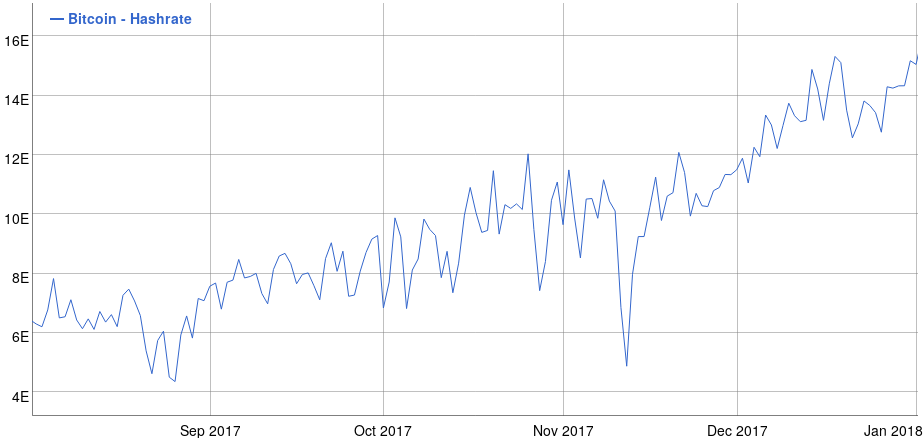
\includegraphics[width=200pt]{img/btc-hashrate-aug2017-jan2018.png}
		  \captionof{figure}{BTC hash rate (late 2017)}
		  \label{fig:btchashrate2017}
		\end{minipage}%
		\begin{minipage}{.5\textwidth}
		  \centering
		  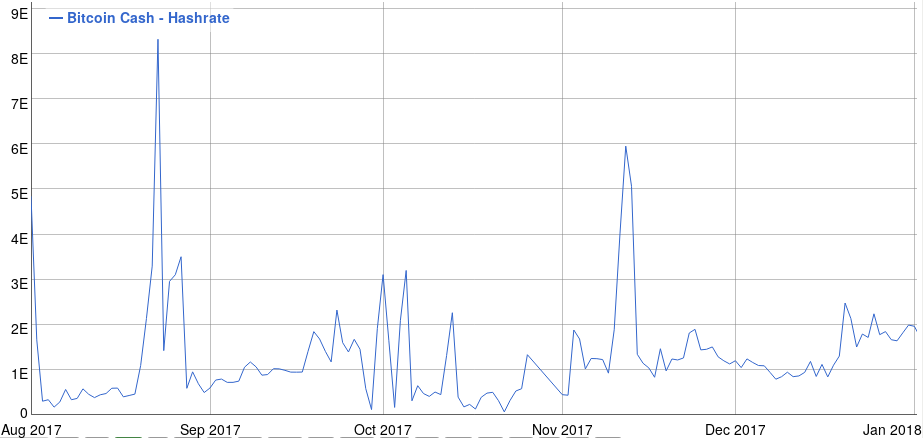
\includegraphics[width=200pt]{img/bch-hashrate-aug2017-jan2018.png}
		  \captionof{figure}{BCH hash rate (late 2017)}
		  \label{fig:fig:bchhashrate2017}
		\end{minipage}
		\end{figure}
		For the rest of 2017 The big-blocker community attempted to coerce miners into mining Bitcoin Cash instead of Bitcoin using another method: market manipulation. \index{Market manipulation} Exchanges \index{Exchange} began to offer BCH trading \index{Trading} and as soon as this happened, big-blockers began to unload millions of dollars of BTC into the free market and buy up BCH, inflating its price. Due to its comparatively low hash rate, some miners switched their hashing power to mine BCH instead of BTC, as soon as it became more profitable to do so. These ``pumps" were also strategically timed to happen right after BTC difficulty \index{Difficulty} adjustments, meaning BTC would lose a large chunk of hashing power right after having its difficulty set to high, making it go even slower, causing transactions to pile up. During this time, the cryptocurrency market was in its biggest bubble \index{2017 bubble} ever, so the Bitcoin chain was already abnormally busy and congested. The large, sudden drops in hash power caused transaction costs to soar, with people paying hundreds of satoshis per byte for block space, often waiting hours or days for a confirmation. \\
		
		For a brief period in November 2017, the BCH \index{BCH} hash rate did surpass the BTC hash rate \index{Hash rate} and many people thought it was the beginning of the end for Bitcoin, but as soon as enough hash power poured into BCH that it became unprofitable to mine, \index{Mining} miners flocked back to BTC. Ultimately BCH failed to ``become" Bitcoin and remains Bitcoin Cash. After the crash of 2018, BTC hash power continued to rise steadily while BCH hash rate stagnated. Interestingly, the peak BTC price in late 2017 coincided almost exactly with the daily transaction limit of $432,000$. \\
		
		\subsection{The Lightning Network}
		
		In February 2015, Joseph Poon and Thaddeus Dryja published a draft whitepaper for a proposed scaling solution they called \textit{The Lightning Network} (LN) \index{Lightning Network} \cite{ln}. The LN would scale Bitcoin but in a very different way from Bitcoin Cash. \index{Bitcoin Cash} There would be no fork and the underlying cryptocurrency would remain BTC. The Lightning Network was to be a \textit{layer-2} protocol, meaning LN made calls to Bitcoin, but Bitcoin was not aware of LN. This meant development of Bitcoin Core \index{Bitcoin Core} and LN could continue on separate tracks. \\
		
		LN worked by moving the majority of payments off-chain to a graph \index{Graph} of users, interconnected by \textit{payment channels}. \index{Payment channel} A payment channel between two users, Alice and Bob, consists of two Bitcoin transactions and a private bidirectional communication channel between Alice and Bob. To open a channel, Alice and Bob each pay some Bitcoin into a single transaction known as the \textit{funding transaction} \index{Funding transaction (LN)} which is broadcast to the Bitcoin network. Once confirmed, the amounts paid by Alice and Bob show up on the LN as \textit{channel capacity}. \\
		
		
		A second transaction known as the \textit{commitment transaction} \index{Commitment transaction (LN)} is created by the LN, which spends both outputs of the funding transaction, giving Alice and Bob back their money. However the commitment transaction is not broadcast \index{Broadcast} to the Bitcoin network, but shared privately between Alice and Bob and keeps track of how much of the channel capacity currently belongs to each of them. To change it, they must both sign an updated version of the commitment transaction. \\
		
		Alice and Bob may open many payment channels with many other users, forming a graph. If Carol wants to pay Alice but only has a channel open with Bob, Carol will pay Bob then Bob will pay Alice the same amount, meaning effectively Carol has paid Alice without being directly connected to her. This is achieved in a trustless way using \textit{hashlocks}\cite{hashlock}, \textit{timelocks}\cite{timelock}, and \textit{hashed time locked contracts}\cite{htlc}. \\
		
		The LN captured the imagination of the Bitcoin community, and through a combination of hard work, meticulous protocol design, and community involvement grew from a set of technical specifications to a fully-realized payment network with over 10,000 \cite{lnstats} nodes.
		
	\section{Problems With These Attempts}
	
	\textit{Bitcoin Cash} \index{Bitcoin Cash} \index{BCH} and \textit{The Lightning Network} \index{Lightning Network} are two very different attempts to scale \index{Scaling} Bitcoin, made for arguably different reasons and for a different set of customers, each with its own pros and cons. \\
	
		Bitcoin Cash achieves the goal of scaling the block size limit \index{Block size limit} but not on the Bitcoin blockchain. Since Bitcoin Cash is a hard fork \index{Hard fork}\index{Fork} its ``scaling improvements" are not enjoyed by Bitcoin, since the miners \index{Mining} ultimately voted to reject them, making Bitcoin Cash \index{Bitcoin Cash} \index{BCH} a breakaway project. However, if Bitcoin Cash's big-block idea had been accepted by the community, it still would have created problems. If the 1Mb limit was removed, and BTC blocks were allowed to grow boundlessly, new nodes coming online would take longer to sync \index{Syncing} and require more storage space. This means it would be no longer feasible to run a full node on a low-power device such as a laptop, and nodes would require ever more expensive hardware on which to run. This would result in centralization. \index{Centralization} \\
	
		Another potential risk of removing the cap is blockchain bloat. Some Bitcoin users have found an alternative use for its blockchain as a persistent datastore. If fees were kept low (as in the sales pitch of the big blockers), it would make sense for businesses to store data on the blockchain instead on on-premises or in the cloud. \index{Cloud} For example, if block space costs $\$0.00001/byte$, it would cost only 3 cents to store 1Gb of data, with free unlimited reads, forever. If this were to happen, miners would face increased costs due to the bloat in the size and volume of transactions, and would be forced to engage in price fixing: \index{Price fixing} not accepting transactions below a minimum fee level. If the blockchain grew to a similar size due to organic adoption, miners would face the exact same problems. Nodes would also take longer to sync and require more expensive hardware. \\
		
		Even if Bitcoin Cash solved the block space issue perfectly and the solution was accepted by the Bitcoin community and integrated into Bitcoin core, the problem of slow transactions still remains. Buying a cup of coffee would be cheap but you may have to take your coffee cold, as the transaction would still take 10 minutes to confirm. The Lightning Network was designed with this specific use-case in mind: Transactions on LN are very cheap and very fast, and it has an in-built invoicing system so the coffee shop sends you an invoice, it shows up on your Lightning wallet no matter which wallet you're using since it's part of the protocol, and you tap on the screen of your device to pay the invoice. Since the LN is a graph, and the complexity of any one node is limited to its interactions with its peers, one would think that LN could scale boundlessly in a similar way to the internet. However LN has some intrinsic design flaws, some of which require added infrastructure and complexity, and others which are not fixable.
	\subsubsection{Onboarding 1 Billion Users to The Lightning Network} \index{Onboarding}
	As of 2020, an estimated $1.6$ billion people use Facebook \cite{fbusers} \index{Facebook} and $441$ million people use Apple Pay \cite{apusers}. \index{Apple Pay} These numbers are continuing to grow, so its not unreasonable to assume that a global digital payment network such as LN could have a potential user base of 1 billion people; if not now, certainly in 10 years time. To calculate how long it would take to onboard 1 billion users to the LN, we first make some conservative assumptions:
	\begin{enumerate}
		\item Each user has exactly 3 payment channels
		\item Once open, a payment channel is never closed
	\end{enumerate}
	Since each user has 3 channels and there are 1 billion users, that makes $\frac{3 \times 1,000,000,000}{2} = 1,500,000,000$ channels, which requires that $1,500,000,000$ funding transactions be broadcast to the Bitcoin network and included in blocks. Since the Bitcoin chain can handle 5 TPS, this will take $\frac{1,500,000,000}{5} = 300,000,000 $ seconds, or 9.51 years - consuming the entire capacity of the Bitcoin network for nothing but LN funding transactions.
	\subsubsection{The Need To Buy Capacity}
	If Alice is organizing a big event where she's expecting 10,000 attendees and charging 0.01 BTC per ticket and wants to receive payment for the tickets over LN, she needs to ensure that her payment channels have a total of at least $0.01 \times 10,000 = 100$ BTC, otherwise she will not be able to receive payment for all the tickets. This requires Alice to manually check the capacity of her payment channels, and if there is not enough capacity \index{Capacity (LN)} in those channels, she will need to open more channels until there is enough capacity, costing Alice time and money. If any of the channels are closed while she is receiving the payments, she runs the risk of running out of capacity, so in fact, she may need to open more channels so she has some ``cushion". While Alice is waiting for the payments, the money in these channels is sitting idle and could probably be put to better use by the counterparties, such as loaning or investing, therefore its likely they will charge a high LN fee to each payer. If Alice instead chooses to open many small channels in the hope that the LN fees will be lower, she will have to pay more in Bitcoin fees for the funding and closing transactions. In short, Alice needs to \textit{buy} the ability to receive large payments.
	\subsubsection{The Need For Payees To Be Online}
	A LN transaction requires both the payer and payee to be online at the same time, making it a synchronous protocol. \index{Synchronous protocol} Failure to be online can result in failed payments or the need to keep re-trying a payment until it succeeds. This makes LN ``spotty", and consequently unreliable. Furthermore, users need to remain online to monitor their payment channels \index{Payment channel} in case a counterparty \index{Counterparty} decides to close a channel. \index{Closing (payment channels)} This need for constant monitoring makes LN infeasible for use in places with poor internet connectivity, on mobile devices, or in any scenario without continuous uptime.
	
\chapter{The Solution}
	\section{Analytical Work}
	As I began this project, I had a clear idea of what I wanted the end result to be (and not to be). I was \textbf{not} making a new cryptocurrency or inventing some radical new use-case. Rather, I was solving a problem: the problem of slow and expensive Bitcoin transactions. Once the problem was solved, people could keep using Bitcoin as before, only faster and cheaper. Having this in mind allowed me to treat the project purely as an engineering exercise. \\
	 
	To get ideas, I began by taking a look at some blockchain projects which had already delivered what they describe as high transaction throughput. The first project I looked at was \textit{Nano}, formerly \textit{RaiBlocks} \cite{nano}. I downloaded the Nano whitepaper and began reading about how it worked. Nano's developers claim to have achieved 105.75 sustained TPS with a peak of 306 TPS. \cite{nanowiki} Although not Visa-level, this sounded impressive, and the other impresive thing about Nano was its instant, feeless transactions. \\
	
	I read about how Nano achieves this: each address (or \textit{account}) on the Nano network has its own blockchain which is hosted on the device of the account owner. When Alice wants to send Bob some $NANO$, she appends a \textit{debit transaction} to her chain, then broadcasts the associated \textit{credit transaction}, which Bob later picks up and appends to his chain.  \\
	
	Each transaction is overseen by a \textit{representative}, who's job is to detect and resolve double-spends. \index{Double spend} A representative's \index{Representative (Nano)}influence is proportional to the amount of $NANO$ they hold in their account, making Nano a proof-of-stake \index{Proof-of-stake} cryptocurrency. It has a one-transaction-per-block model, which I thought was better than Bitcoin's design of many transactions per block, because it imposes a transaction-level ordering. \\
	
	I wondered how Nano \index{Nano} achieved feeless transactions, since \textit{feeless} meant it was free to send spam transactions. After some digging, I learned that Nano's spam protection was achieved by having the sender compute a small proof-of-work before being allowed to send their next transaction. I thought about the idea of making \textit{Conclave} feeless, which would certainly make a good selling-point, but Nano seemed to leave some unanswered questions: For example if Alice pays Bob while he's offline, then Alice goes offline, how is Bob guaranteed to receive the credit transaction from Alice when he comes online? During this period, Alice's chain is debited but Bob's is not yet credited, so the representatives need to ensure Bob gets the transaction when he comes online. I could not find an answer in the whitepaper as to how delivery was guaranteed on the Nano network. \\
	
	I thought about what kind of blockchain Conclave would have, and I settled on the idea of a traditional single, shared blockchain but I wanted it to be scalable and for that to happen it would need to be allowed to grow to a size such that it would not all fit on one machine. This would require splitting the blockchain across several nodes - a technique known as \textit{sharding}. However sharding brings its own set of questions:
	\begin{itemize}
		\item How to distribute the data?
		\item How to ensure malicious nodes don't tamper with blocks?
		\item How to ensure that at least one node has every piece of the blockchain?
	\end{itemize}
	
	I took a look at some more blockchain projects to see if I could find answers to these questions and get more ideas. To try answer the questions about data storage I took a look at \textit{Siacoin} \cite{sia}. Siacoin \index{Sia} is the cryptocurrency of the Sia network, which is a decentralized storage network, aimed at customers who require decentralized file storage. \\
	
	Users wishing to participate in the Sia network download and set up the Sia node software, allocating a portion of their hard drive space to the Sia network, and get paid in Siacoin for keeping their node running. The more space they allocate, the more Siacoin they earn. I was curious about how this network worked and how it protected against dishonest participants pretending to have more space than they did, or deleting the files then pretending that they still had them. I read through the Sia whitepaper and learned that Sia uses a system of \textit{storage contracts} \index{Storage contract (Sia)} to protect itself against these risks. \\
	
	A Sia participant, Alice, who needs a file stored will enter into a storage contract with another Sia participant, Bob, who agrees to store that file for Alice for a certain length of time in exchange for an agreed fee, and during this time Bob must regularly publish proofs to the Sia blockchain that he is continuing to store this file. This is achieved using a decentralized random number generator which chooses a small part of the file which Bob must publish to the blockchain, together with a list of hashes from the file's Merkle tree. If Bob fails to do this, he will not get paid. If he publishes an incorrect proof, other participants who are storing the same file could dispute it, and take Bob's payment, motivating Bob to behave honestly. This gave me some ideas as to how to ensure the Conclave blockchain would stay intact and parts of it wouldn't go missing. \\
	
	Next, I began to think about how Conclave nodes would achieve consensus among themselves on the ordering of transactions. If transactions $B$ and $C$ both spent from transaction $A$, how to decide which one ``wins" ? $B$ may have happened before $C$ from Alice's perspective, but perhaps not from Bob's perspective. In a decentralized network spanning the Earth, time is relative, and issues such as clock skew, network latency, and the potential for nodes to behave dishonestly make this a hard problem. \\
	
	I took a look at \textit{Hedera Hashgraph} \cite{hedera}, \index{Hedera Hashgraph} a project which went live in late 2019. Hedera Hashgraph is a permissioned public ledger designed for enterprises. It can be used to store arbitrary transactions including banking transactions and stock trades: transactions where an accurate timestamp is essential for legal reasons. One of Hedera's selling points is that each transaction has a ``fair and accurate" timestamp, which leads to fair and accurate ordering. I read through the Hedera whitepaper to find out what they mean by ``fair and accurate", and how it is achieved. \\
	
	On the Hedera network, a transaction is broadcast to the network by an originator, and upon receipt of the transaction, each node attaches a timestamp \index{Timestamp} to the transaction indicating when they first saw the transaction, then passes it on to their peers. Each node's timestamp constitutes a vote, \index{Voting} and the median of the votes becomes the official timestamp of the transaction. \\
	
	This seemed like a simple but effective way of timestamping and ordering transactions, since it was forgiving of small inaccuracies in the clocks of honest nodes, and resistant to deliberate attempts to skew the timestamp by malicious nodes, provided the majority of the nodes were not malicious. I could use this method to ensure a deterministic ordering of transactions provided I had a way of preventing malicious groups of nodes from creating false timestamps - an attack known as a \textit{sybil attack}. \index{Sybil attack} \\
	
	Having got these ideas and inspiration from other projects, I set to work on building Conclave.
	
	\section{Architectural Level}
		\subsection{Network Architecture}
		\textit{The Conclave Network} consists of a graph of \textit{Conclave nodes}, each running a dæmon program called \texttt{conclaved}. Each \texttt{conclaved} \index{conclaved} instance performs the following tasks:
		\begin{enumerate}
			\item Servicing requests from users who want to check their balance or send new transactions
			\item Relaying transactions to and between peers
			\item Verifying, timestamping and sequencing transactions
			\item Putting transactions into blocks
			\item Storing blocks on the Conclave blockchain
			\item Relaying blocks to and between peers
		\end{enumerate}
		These six tasks can be further distilled down to two:
		\begin{enumerate}
			\item Servicing requests from users
			\item Storing and updating the blockchain
		\end{enumerate}
		Each node runs an RPC service which any user may connect to, without needing permission, and interact with the Conclave network, typically checking their balance and sending transactions. No trust is required between the user and the node. A malicious node can send the user false information but can not take their money. Each node's RPC service can be thought of as an ATM machine that's guaranteed not to be compromised.  \\
		
		The network is designed in so that no single node is required to be online for the network to function, and the network can scale its transaction throughput simply by scaling the number of nodes. The Conclave blockchain is sharded across the network.
		
		
		\begin{figure}[H]
			\begin{center}
				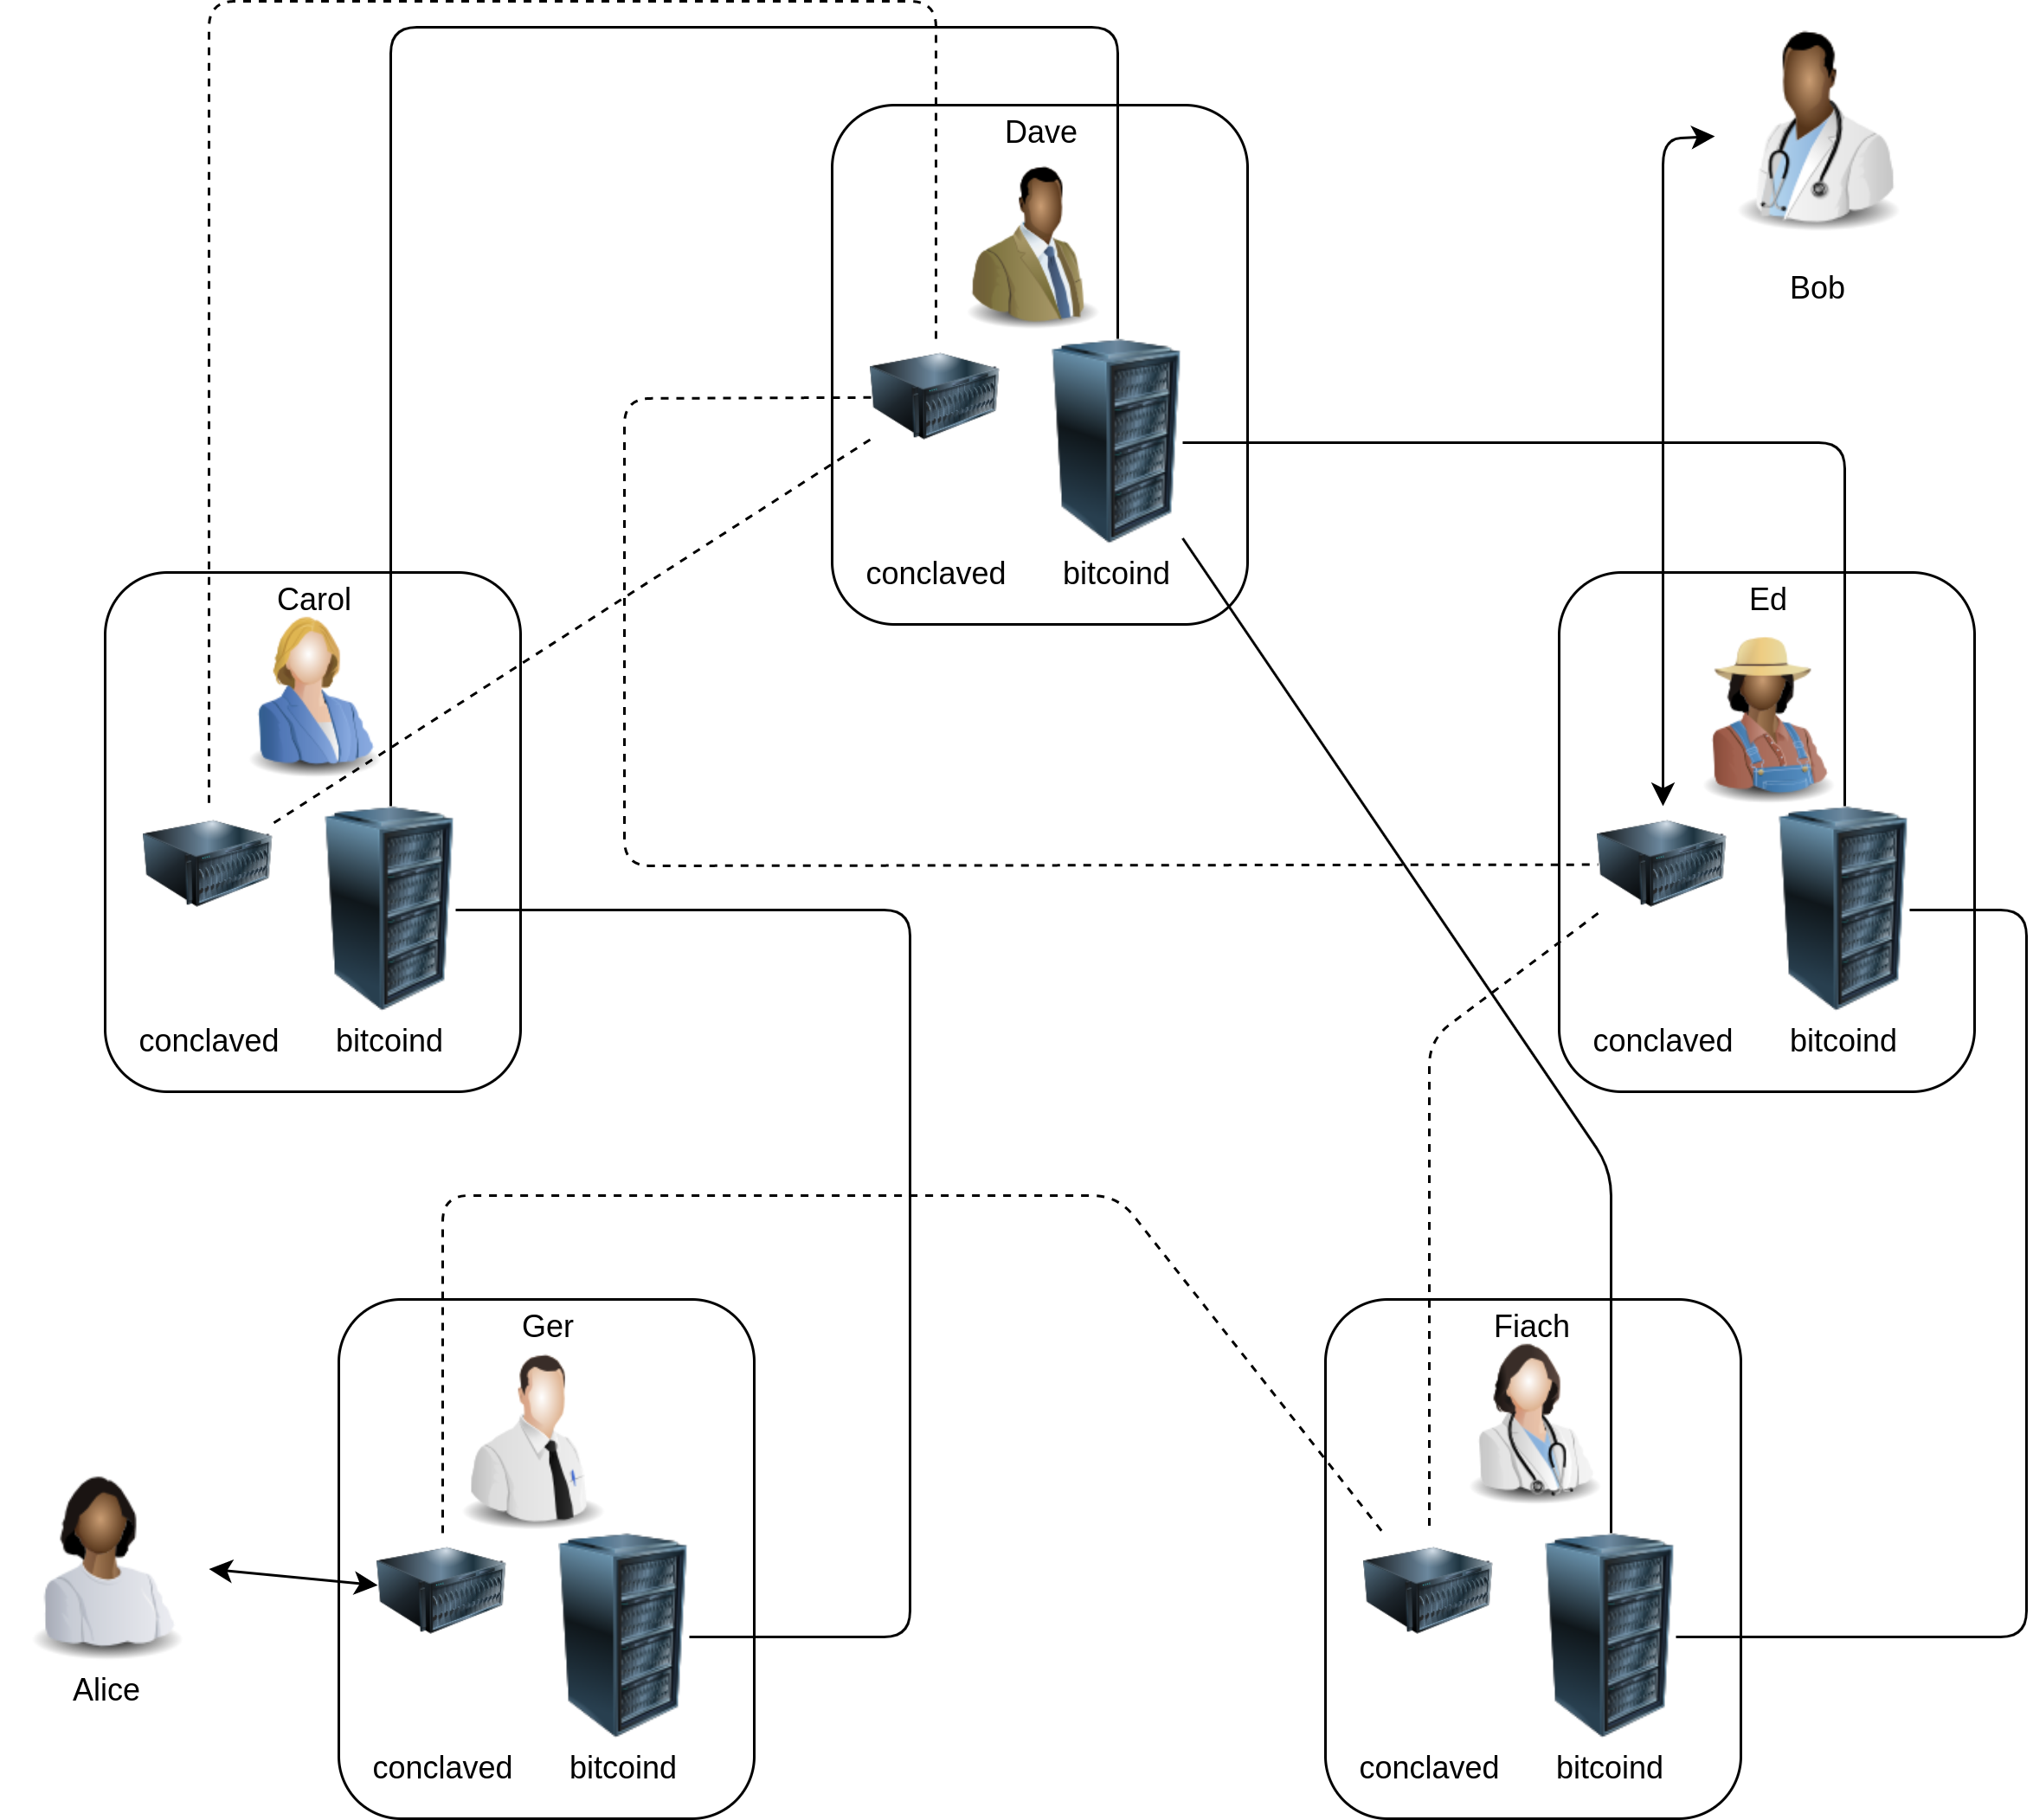
\includegraphics[width=250pt]{img/ConclaveNetwork.png}
			\end{center}
			\caption{The Conclave Network}
			\label{fig:conclaveNetwork}
		\end{figure}
		
		
		\subsubsection{Relationship to Bitcoin}
		The Conclave network is built on top of the Bitcoin network, therefore each \texttt{conclaved} node is required to have its own \texttt{bitcoind} node, with an independently-verified copy of the Bitcoin blockchain. The Conclave chain tracks and references the Bitcoin chain and each Conclave block contains the hash of the most recently mined Bitcoin block. \\

		
		\begin{figure}[H]
			\begin{center}
				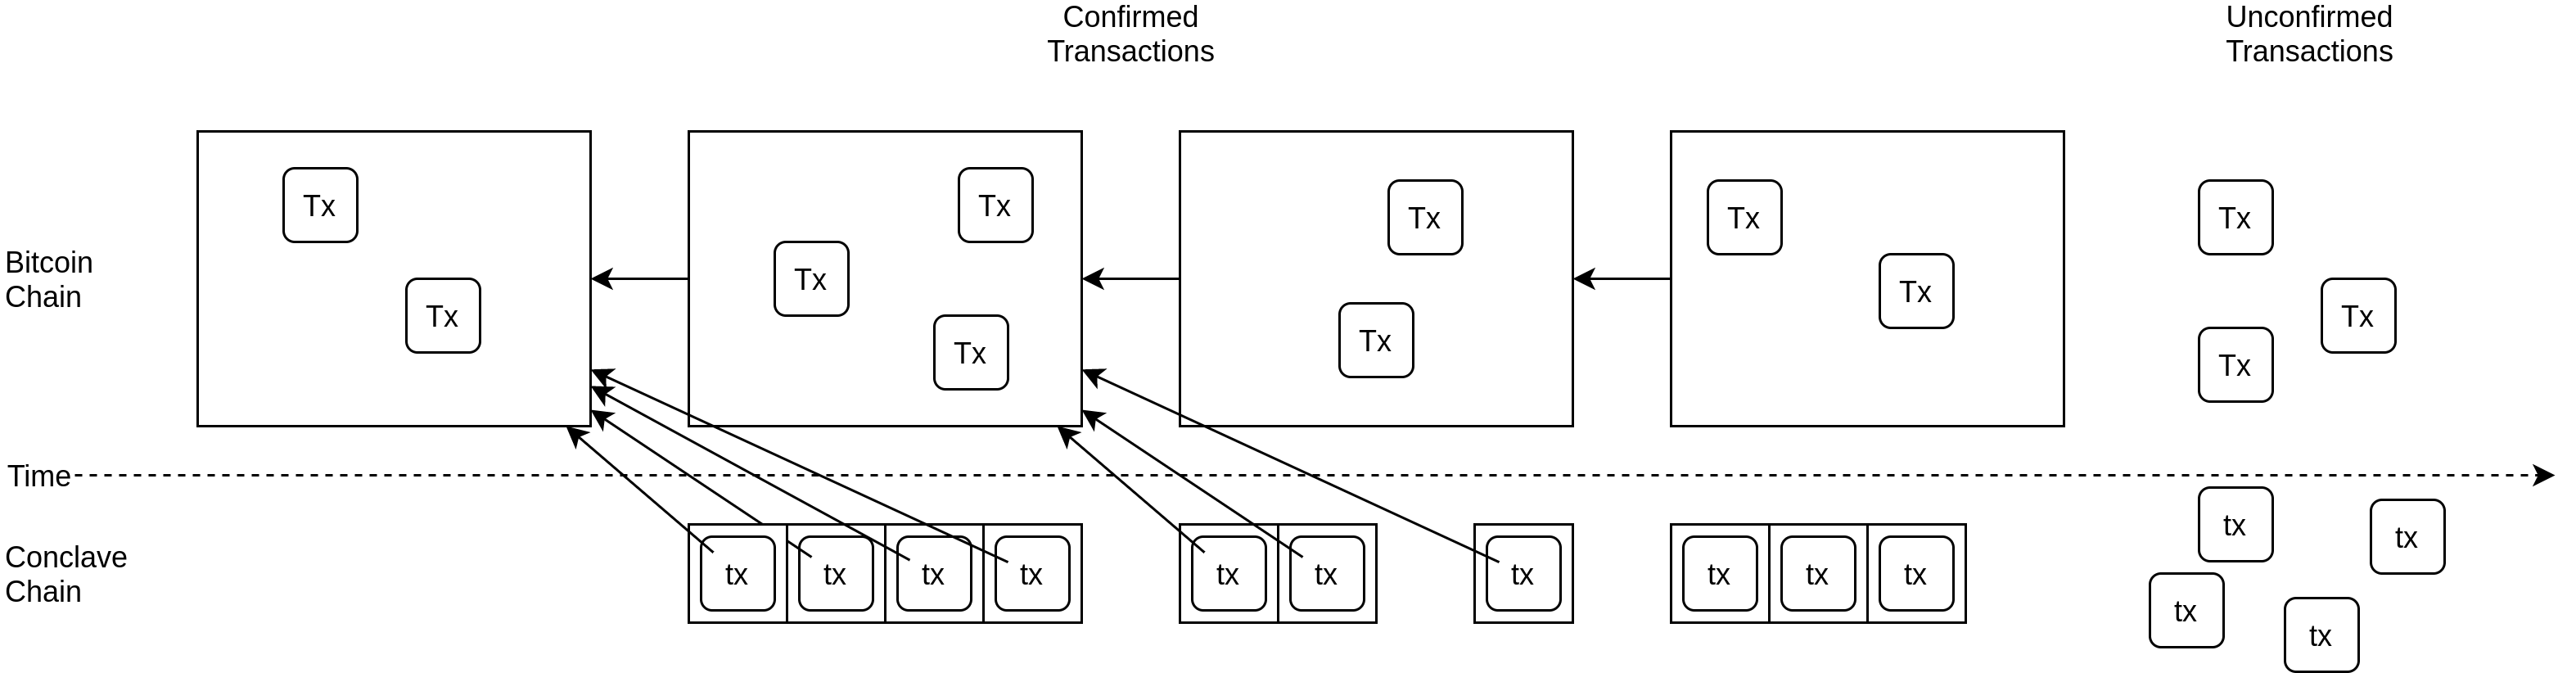
\includegraphics[width=400pt]{img/2Blockchains.png}
			\end{center}
			\caption{The Conclave and Bitcoin Blockchains}
			\label{fig:conclaveAndBitcoin}
		\end{figure}
		
		Unlike Bitcoin blocks, which can contain zero or more transactions, each Conclave block contains exactly one transaction. If there are no transactions pending, no block will be created. When a transaction is broadcast to the Conclave network, the transaction is endorsed, timestamped, and sequenced, and the block is created as quickly as possible. Unlike Bitcoin, no proof-of-work is required.
		\subsection{Bootstrapping the Network}
		The Conclave network and blockchain rely on the Bitcoin network and blockchain to store system data essential to the security and smooth-running of the Conclave network. Over time, small ``checkpoints" are published to the Bitcoin blockchain which define how the node should behave. A bootstrapping Conclave node reads the entire history of these checkpoints to get a full history of the state up to the current state. 
			\subsubsection{Network Parameters}
			The Conclave \textit{network parameters} are a set of shared variables which control how the Conclave network operates. The network parameters have extremely strong consistency backed up by the hash power of the Bitcoin blockchain. The network parameters can be adjusted with a special transaction appearing on the Bitcoin blockchain known as a \textit{network parameter adjustment transaction} (NPAT). An NPAT can be created by anybody, but must be \textit{community signed} in order to be officially recognised by a node.\\
			
			Future versions of the Conclave protocol may add or remove network parameters. For V1, the following network parameters are defined: \\
			
			\begin{center}
			\bgroup
			\small
			\def\arraystretch{1.5}
			\begin{tabular}{|l|l|l|}
			\hline
			\textbf{Name} & \textbf{Type} & \textbf{Purpose} \\ \hline
			\texttt{minTrust}             & Real             & The minimum summed trust score required for a valid endorsement \\ \hline
			\texttt{maxEndorsers}             & Integer             & The maximum number of endorsers allowed on a valid endorsement \\ \hline
			\texttt{multiSigN}             & Integer             & The number of public keys required in a multisignature (the \textit{n} in m-of-n) \\ \hline
			\texttt{potPayoutLevel}        & Integer             & The number of satoshis the pot must contain before a payout is triggered \\ \hline
			\texttt{blacklist}            & \{PublicKey\}             & The set of public keys which have been blacklisted  \\ \hline
			\end{tabular}
			\captionof{table}{Conclave Network Parameters}
			\egroup
			\end{center}
			
			
			\subsubsection{Iception Transaction}
			
			The \textit{inception transaction} is the first NPAT, and a special NPAT, insofar as it nominates the first node who may be trusted, however this node will have an initial trust score of zero.
			
		\subsection{Proof-of-Trust (PoT)}
		Every blockchain needs a trust system to ensure fairness and honesty and to make cheating either impossible or prohibitively expensive. Early blockchains including Bitcoin use \textit{proof-of-work (PoW)}, which involves repeatedly computing hashes until a certain number is found. Newer blockchains including NEM and EOS use \textit{proof-of-stake (PoS)} which pays stakers, who put a large amount of their own capital at risk, to verify transactions, with the risk of losing their stake if they behave dishonestly. 

The trust system upon which Conclave is built is called \textit{proof-of-trust}, or \textit{PoT}. $PoT$ incentivises nodes to be online as much as possible, to provide a quality service, and not to engage in dishonest behaviour. It does not require large amounts of compute and electricity, or large amounts of money.
		\subsubsection{Earning Trust}
		Each participant has a positive real number associated with it known as its \textit{trust score}.  The trust score for a node $N$ is calculated by the formula:
		\[trust_N = \sum_{i=1}^n\frac{1}{t_i - t_0}\]
		Where:
		\begin{itemize}
			\item $n$ is the number of Conclave-compliant multisignature spends $N$ has signed in its lifetime
			\item $t_i$ is the time when UTXO $i$ was created (the $i$th UTXO for which $N$ was a trustee)
			\item $t_0$ is the timestamp of the inception transaction 
		\end{itemize}
		
		
		
		\subsubsection{Earning Trust} \index{Trust}
		The amount of money a node earns is directly proportional to its trust score. The only way nodes can earn trust is to sign \textit{withdrawal transactions} on the base blockchain. To be eligible to sign a withdrawal, the node must first be one of the m \textit{trustees} of a \textit{funding transaction}. Any node that is a trustee has the chance to increase its trust score whenever the opportunity arises to sign an exit transaction, therefore are motivated to stay online and do so.
		\subsubsection{Losing Trust}
		A node's trust score can stay the same or increase, but never decrease. If a node breaks any of the \textit{trust rules}, it will lose all its trust points and be blacklisted.
		\subsubsection{Trust Rules}
		The \textit{trust rules} are a set of rules which, if broken by a participant, result in that participant being blacklisted. Breaches of the trust rules include:
		\begin{itemize}
			\item Spending a UTXO outside of the rules of the protocol.
			\item Sending provably false information to a peer or to a client.
			\item Attempting to claim a reward with a false \textit{proof-of-storage}.
		\end{itemize}
	
		\subsubsection{Community Signing} \index{Community signature}
		\textit{Community signing} is the process by which a subset of the Conclave network participants collectively endorse a message. More exactly, a message $M$ is said to be \textit{community signed} by a set of $n$ participants $P$, at a time $t$, if a set of $n$ signatures of $M$, $S_M$, each signed by a different member of $P$, exist such that:
		
		\[ \sum_{i=1}^n trust_{{p_i}_t} \ge minTrust, n \le maxEndorsers, p_i \in P \]
		
		A set of $n$ such signatures is known as a \textit{community signature}. Choosing sensible values for \textit{minTrust} and \textit{maxEndorsers} ensure that community signatures cannot be made which include many signers with low trust scores.
		
		\subsubsection{Blacklisting} \index{Blacklisting}
		If a node is blacklisted, its trust score is reduced to zero and the node may no longer participate in the Conclave network. A blacklisted node may not be named as a trustee for any future deposit transaction, but still may sign withdrawal transactions for which it was a trustee, but will earn no trust points. Once blacklisted, a node can not be un-blacklisted.
		
		\subsubsection{Self-Blacklisting}
		A node may blacklist itself without breaking any of the trust rules by signing a message stating that it wishes to do so, and broadcasting it. Any node intending to cease participation in the Conclave network for good \textit{should} blacklist itself, although it's not essential. Nodes that become inactive will quickly be noticed and not selected as trustees. Another reason a node may wish to blacklist itself is if its private key is compromised.
		
		\subsubsection{Non-Transferability of Trust}
		Trust points are strictly non-transferable. \index{Transferability} This is a deliberate design decision which aims to curb centralization. \index{Centralization} Since every node's trust score is intrinsically tied to its private key, transferring ownership of that trust implies transferring ownership of the private key - which cannot be done with any confidence as the sender must somehow convince the receiver that they have erased their knowledge of the private key and not divulged it to anybody. \\
		
		If trust points were transferable, network centralization and possible network corruption are almost sure to occur since well-funded parties are likely to ``buy out" \index{Buyout} high-trust nodes in order to grow bigger. Non-transferability of trust means trust cannot realistically be bought, just as real trust cannot be bought, but instead must be earned through consistent positive contributions to the network in the form of high uptime and honest behaviour.

		\subsection{Trustees}
			When a user sends some bitcoin from a classic address to a Conclave address, the bitcoin appears to the user to move off the Bitcoin chain and onto the Conclave chain, however it never really leaves the Bitcoin chain, but rather goes out of control of the sender and into the control of a set of Conclave participants who control the destination UTXO. \index{UTXO} This UTXO is then said to be \textit{Conclave-controlled}, and the $n$ participants whose public keys control the UTXO are the \textit{trustees}. Trustees are Conclave participants whose public keys appear in the locking scripts of Conclave-controlled UTXOs. \\
			
			A trustee of a UTXO is any participant who is a signatory on such a script and have thereby been trusted, as a member of a group, to take care of that UTXO and the value contained therein, for the depositor. When the depositor wishes to send the bitcoin back to their Bitcoin address (i.e. to \textit{withdraw}), at least m of the n trustees need to sign a transaction which spends this UTXO, sending it back to the user's Bitcoin address, although it's unlikely that it will be from the same UTXO that they deposited to. The Conclave network takes care of the book-keeping to ensure there is enough bitcoin available in Conclave-controlled outputs to honour their withdrawal.\\
			
			\textit{It can be tempting to refer to any network participant as a ``trustee", \index{Trustee} however the word should be reserved for occasions where the participant is acting in their capacity as a trustee of a particular Conclave-controlled output.}
		\subsection{Rewards}
		Each Conclave transaction collects a minimum fee of 1 satoshi and each block includes a field called the \textit{pot}, \index{Payout} which is a running total of collected fees. When the pot reaches the \textit{pot payout level} (defined in the \texttt{potPayoutLevel} network parameter), \index{Network parameter} \texttt{potPayoutLevel} satoshis are moved from the pot into the \textit{unclaimed pot}, and all network participants may claim a share of this payout proportional to their trust score, \index{Trust score} before the pot fills again. When the pot again reaches \texttt{potPayoutLevel}, any remaining unclaimed funds are moved from the unclaimed pot back into the pot. \\
		
		Any node who fails to collect their reward before the pot refills forfeits their payout for that cycle. Rewards \index{Reward} do not ``carry over", so nodes are incentivised to stay online and actively collect their reward each cycle. To collect their reward, a node must complete a small task called a \textit{proof-of-storage}, then they may broadcast a transaction which spends any amount up to their share from the unclaimed pot to their primary address. If they claim less than they're entitled to, the unclaimed satoshis remain in the unclaimed pot and may not be claimed by anybody else. \\
		
		Blocks where the \texttt{potPayoutLevel} threshold is reached are known as \textit{payout blocks}. \index{Payout}
		
		\subsection{Proof-of-Storage (PoS)}
		To keep the Conclave blockchain at a high level of durability and responsiveness, nodes are incentivised to store as much of the blockchain locally as they can. When a node with non-zero trust wishes to collect their reward, they broadcast a transaction transferring their claim into their address, together with the solution to a challenge known as a \textit{proof-of-storage}. \index{Proof-of-storage} The challenge \index{Challenge} is to prove that they possess a block from somewhere in the history, whose height is determined by:
		
		\[ (\textrm{SHA256}(B_p) \oplus \textrm{SHA256}(pubkey)) \textrm{ mod } h_{B_p}  \] Where:
		
		\begin{itemize}
			\item $B_p$ is the most recent payout block.
			\item $pubkey$ is the public key of the node being challenged.
			\item $h_{B_p}$ is the height of $B_p$.
			\item $\oplus$ is the bitwise exclusive-or operator, \index{Exclusive-Or} the result of which is interpreted as a binary-encoded unsigned integer.
		\end{itemize}
		
		A node who attempts to claim their reward using an incorrect PoS may be blacklisted. \index{Blacklisting}
		
		\subsection{Blockchain Architecture}
		
		The Conclave blockchain's architecture represents a significant departure from the two most popular models in use today: proof-of-work and proof-of-stake \index{Proof-of-stake} blockchains. The ambition of the Conclave blockchain is to be a next-generation blockchain which has the security of first-generation blockchains, but with significantly improved throughput and confirmation time, making it attractive to end-users, and significantly reduced operating costs, making it attractive to node operators, businesses and enthusiasts. \\
		
		These improvements are built on the foundation of \textit{proof-of-trust}. 
		
	\section{High Level}
		

		\subsection{Transactions}
			The term \textit{transaction} is somewhat overloaded in the world of blockchains. This is doubly true for Conclave since it manipulates two blockchains, each with their own transaction format. To describe how transactions work, I will begin by discussing the practical \textit{actions} which the user wishes to perform: \textit{deposits}, \textit{withdrawals}, and ``regular" payments, and explain how they are implemented in terms of \textit{transactions} on the Bitcoin and Conclave blockchains.
			\subsubsection{Deposits} \index{Deposit}
			A \textit{deposit} is where a user sends bitcoin from the Bitcoin network to the Conclave network. Each deposit involves exactly one transaction on the Bitcoin chain: the \textit{fund transaction} or \texttt{fundTx}, and exactly one transaction on the Conclave chain: the \textit{claim transaction} or \texttt{claimTx}. To make a deposit, a depositor pays a deposit amount $D$ into a P2WSH output, $O$, on the Bitcoin chain and some time later, may claim a value not exceeding $D$ on the Conclave chain, by broadcasting a claim transaction $C$ which proves that $O$ was broadcast with the intention of funding $C$ and $C$ only, and this decision was made before the fund transaction was broadcast. \\
			
			Functionally, a deposit is only concerned with one part of the fund transaction: the fund output, therefore it is possible for a single fund transaction to contain multiple fund outputs - each funding a different claim transaction. However a single claim transaction may only claim one fund output for itself. Each claim transaction includes a pointer to its fund output's location on the Bitcoin blockchain, known as its \textit{fundpoint}. A fundpoint is a standard ``outpoint" structure, consisting of a transaction ID and index. \\
			
			Before a claim transaction is broadcast claiming a particular fund output, the fund output will appear like any other P2WSH output. When the claim transaction is broadcast, together with the fundpoint, this reveals the fund output as such. When a node receives the claim transaction, it fetches the output located at the fundpoint, checks that it is a P2WSH output, then reconstructs the P2WSH redeem script known as the \textit{claim script}. The node then hashes the claim script and checks that the hash matches that of the fund output's \texttt{scriptPubKey}'s P2WSH script hash threby proving that the claim script, and thus the claim transaction, is the rightful claimant of the funds in the fund output. \\
			
			The structure of the claim script is as follows:
			
			\begin{center}
				\texttt{<claimTxHash> drop <n> <trustee 1 pubkey> ... <trustee n pubkey> <m>}
			\end{center}
			
			This is a standard multisignature script with the exception of the first two script elements, which push the \texttt{claimTxHash} on to the stack then pop it. The \texttt{claimTxHash} does not play any role in the logic of the script, however it needs to be there to cryptographically link the script to the claim transaction. Since the \texttt{claimTxHash} is a hash of all the fields of the claim transaction, the claim transaction can not be modified after the fund transaction is broadcast because then it would produce a different hash, breaking the cryptographic link with the fund output. \\
			
			There is no strict deadline imposed on a claimant for claiming a fund output, however if the fund output is very old by the time it is claimed, there may not be enough active trustees from the time it was created still on the network. If the fund output does not comply with the network's trust requirements \textit{at the time of claim}, it needs to be spent into a ``fresh" fund output before the claim is honoured. Once such an output is revealed to the network, the network will immediately try to spend it to a withdrawal transaction, as withdrawal transactions spend outputs in the order they appear in the blockchain, not the order in which they were claimed. However if the network cannot find $m$ active trustees to spend the output, it will be unspendable and the claim is lost.

			
			\begin{figure}[H]
				\begin{center}
					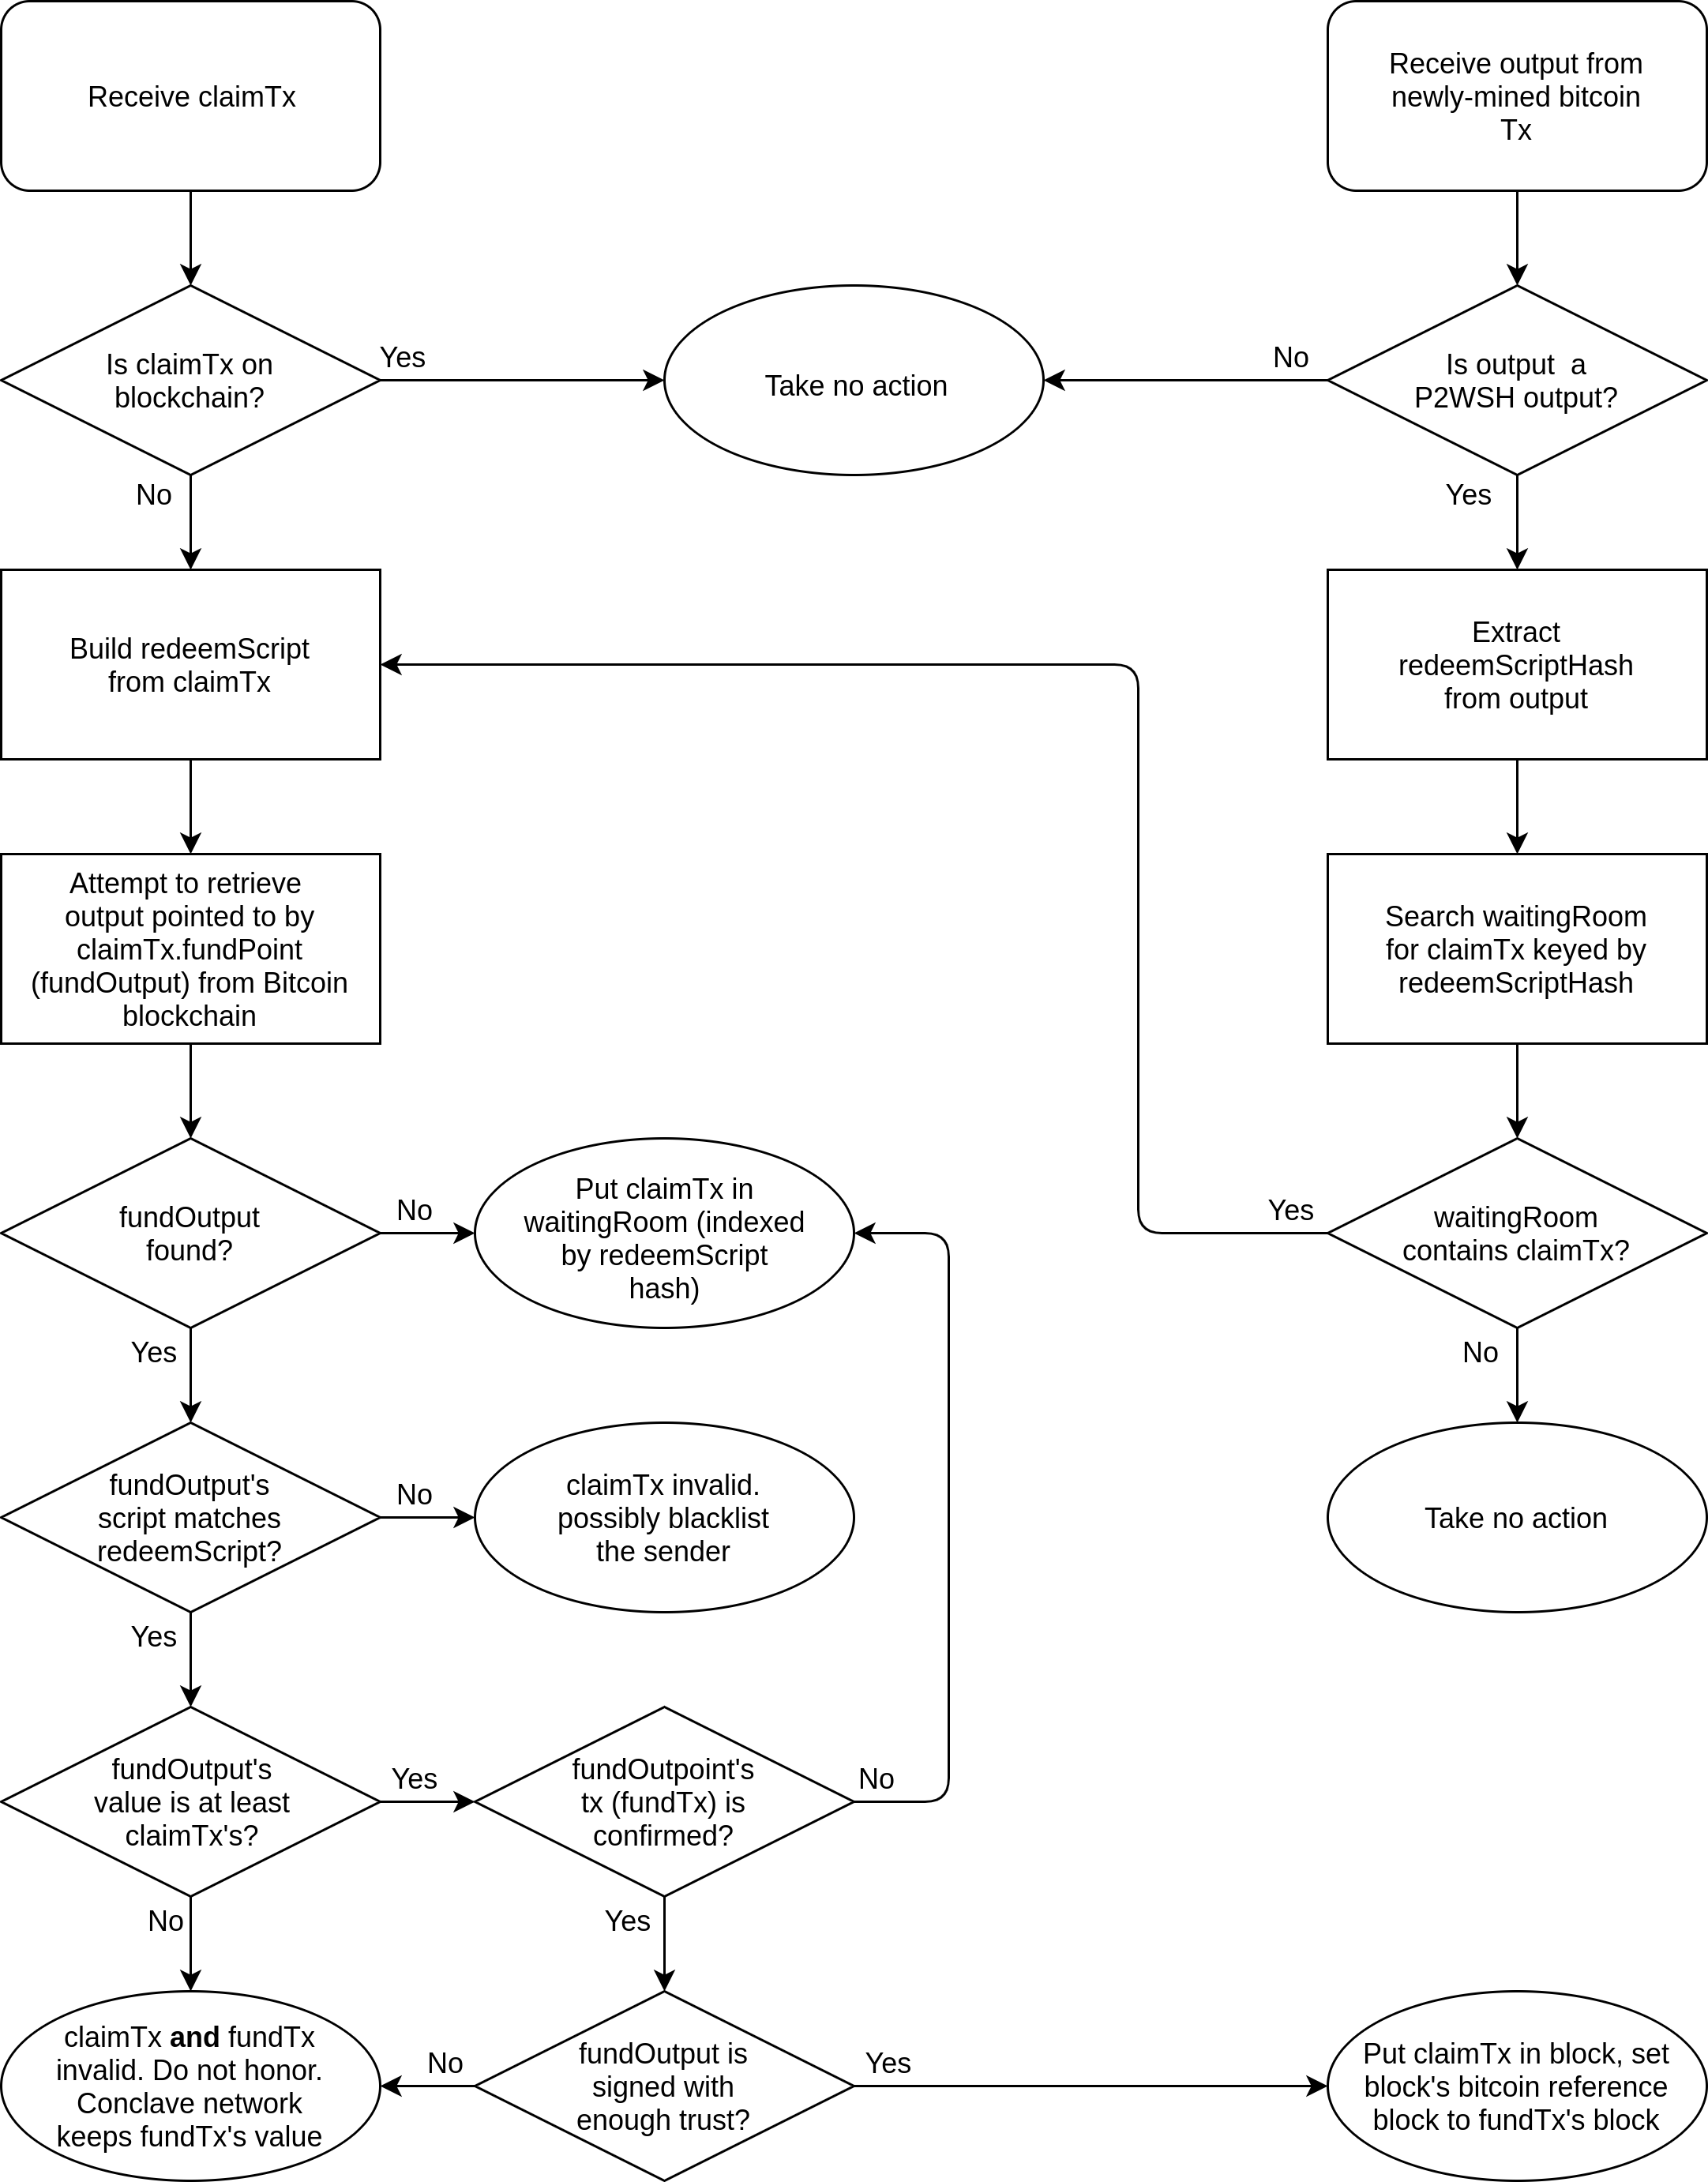
\includegraphics[width=300pt]{img/ClaimTx-flow.png}
				\end{center}
				\caption{\texttt{claimTx} Flow}
				\label{fig:claimTxFlow}
			\end{figure}

			\subsubsection{Withdrawals} \index{Withdrawal}
		
			A \textit{withdrawal} is where a user sends bitcoin from the Conclave network to the Bitcoin network. In terms of transactions, a withdrawal involves exactly one output, known as the \textit{withdrawal output}, and exactly one transaction on the Bitcoin chain known as the \textit{payout transaction}, into which the withdrawal output is copied. A payout transaction can pay out to many withdrawal outputs, and if a Conclave transaction contains many withdrawal outputs, they may land in different payout transactions. \\
			
			Unlike a Bitcoin transaction, a Conclave transaction contains two lists of outputs: \textit{Bitcoin outputs} and \textit{Conclave outputs}. Both lists are structurally identical, however once confirmed on the Conclave blockchain, only the Conclave outputs are spendable on that blockchain. The Bitcoin outputs need to be copied into a Bitcoin transaction, funded, and confirmed on the Bitcoin blockchain at which point they become spendable. \\
			
			Payout transactions are continuously being created and broadcast by Conclave nodes who are scanning the Conclave chain for new withdrawal outputs which require funding, and funding them with the oldest unspent funding outputs on the Bitcoin chain. To make efficient use of Bitcoin block space, payout transactions are made as large as possible, batching many withdrawal outputs together, trying not to create any change outputs. \\
			
			To ensure that no withdrawal output is missed or double-funded, payout transactions are constructed in a way that imposes strict ordering \index{Ordering} rules. Each payout transaction \index{Payout transaction} contains implicit start and end markers denoting the first and last funding output \index{Funding output} it spends, in the order they appear on the Bitcoin blockchain, as well as start and end markers denoting the first and last withdrawal outputs it funds, in the order they appear on the Conclave blockchain. \\
			
			Each time a new Bitcoin block is found, that block will contain exactly one payout transaction, paying out from an ordered range of funding outputs to an ordered range of withdrawal outputs. As soon as this happens, the Conclave network begins working on the next payout transaction, which begins exactly where the previous payout transaction left off. Its first funding output will be the one immediately following its predecessor's last funding output and its first withdrawal output will be the one immediately following its predecessor's last withdrawal output. \\
			
			Immediately after a confirmation there may be very few pending withdrawal outputs, but payout transactions are created, signed and broadcast nonetheless. These will land in the mempool awaiting confirmation, whilst the network continues to make bigger versions of the payout transaction each with the same start markers but growing end markers. The network continues to work on the ever-growing payout transaction until the next confirmation happens, at which point only one of the payout transactions in the mempool succeeds, defining the start markers for the next payout transaction, which the network immediately begins working on.
			
			\subsubsection{``Regular" Transactions}
			
			Any transaction appearing on the Conclave blockchain that is not a deposit or withdrawal, is a ``regular" transaction, and does not involve the Bitcoin blockchain. Regular Conclave transactions have the same mechanics as regular Bitcoin transactions, but are orders of magnitude faster and cheaper and can be made in greater volume.
		\subsection{The Conclave Blockchain}
			\textit{The Conclave blockchain} is the distributed datastore where all Conclave transactions are stored. Although it shares much of its DNA with the Bitcoin blockchain and owes its existence to it, the Conclave blockchain is more advanced and addresses the Bitcoin blockchain's scaling issues. We will now examine these issues and see how the Conclave blockchain solves them.
			\subsubsection{Problems With The Bitcoin Blockchain}
				As of 2020, running a Bitcoin core node requires about 200Gb of disk space, mainly to hold the database files which comprise the blockchain. This is not a major hurdle, but is cumbersome since the entire blockchain must be ``lugged around" with each instance. Also, the initial downloading of data and synching of the blockchain can take a long time - up to several days. \\

				These problems are somewhat alleviated by running \texttt{bitcoind} with a pruned blockchain \index{Pruned blockchain} which can reduce the storage requirement by up to 97.5\% \cite{prune}, however  this compromises one of the core principles of Bitcoin: ``don't trust, verify", because the pruned node must now trust its peers to tell the truth whenever it sees a transaction which references a point in the blockchain before the prune-point. This is still a low risk trade-off in 2020, since nearly all miners' nodes have a full copy of the blockchain, so no invalid blocks will be accepted, but a pruned blockchain also reduces the usability of the node, since it can no longer be used for general purposes such as looking up old transactions and blocks. \\

				As well as this problem of ``bigness" (i.e. requiring 200Gb of free disk space), the Bitcoin blockchain is also noted for its slowness, with each new block taking 10 minutes to be added. This slowness can be attributed to the PoW algorithm. It's worth considering that if everybody behaved honestly and non-greedily, and the difficulty of the Bitcoin blockchain was set to zero effectively eliminating PoW, \index{Proof-of-work} the blockchain would still be valid - the consensus rules would work correctly with value being transferred between addresses and no money getting created or destroyed against the rules. The emission algorithm would work correctly with a halving occurring every 210,000 blocks, and one dominant chain would prevail. \\

				If everybody behaved honestly and only used the blockchain when they legitimately needed to make a transaction, a new block would be mined whenever it needed to be: i.e. when there was one transaction in the mempool awaiting confirmation. If everybody behaved non-greedily, no empty blocks would be mined, even though there was a block reward up for grabs. The result would be a blockchain where there is exactly one transaction per block, the rate of block creation scaled up or down to accommodate the rate of transaction creation, all transactions have would zero confirmation time, and be free. \\

				In such a scenario, a node's disk would fill up very quickly with blockchain data and soon the blockchain would be too big to fit on one disk.
			\subsubsection{Sharding}
				Sharding is a technique for splitting a large dataset into smaller pieces or \textit{shards} and storing each shard on a different machine such that retrieving, adding, updating, and deleting items can still be done in a time comparable to if they were on the same machine. Sharding is heavily used in modern distributed systems and several techniques have been invented for keying and organizing the data. One of the most famous of these is the \textit{distributed hash table} (DHT). \index{Distributed hash table} \texttt{bitcoind} stores the blockchain in a completely unsharded way, meaning every node (with the exception of pruned nodes) has the entiriety of the blockchain stored locally.
			\subsubsection{Redundancy}
				Virtually all modern distributed systems which store data do so in a \textit{redundant} way, meaning multiple copies of the same data are stored on different machines, possibly on different continents, so that if one machine fails, gets hacked, or is siezed by the government, the data will still be available somewhere else. \\

Bitcoin already satisfies this redundancy property, with an estimated 10,000 independently-verified copies of the blockchain residing on nodes around the world, running on systems ranging from smartphones to enterprise cloud systems \index{Cloud} with redundancy guarantees of their own. Many of these services consider 3 replicas of their customers' data to be sufficiently redundant, as do their customers. Since the Bitcoin blockchain has tens of thousands more replicas, it's clear that it over-satisfies the redundancy property.
			\subsubsection{Design Goals}
				Redundancy and sharding \index{Sharding} usually go hand-in-hand because the more sharded a dataset becomes, the more machines that are required to store it, and since every machine has a certain chance of failing, putting the same data on multiple machines reduces the probability \index{Probability} of a specific item of data becoming unavailable. \\

				Together, the techniques of redundancy and sharding affect two properties which are of great importance: \textit{data availability} and \textit{data durability}. Although they are not rigorously defined, these properties are crucial and many methods have been devised to measure them. Roughly speaking, availability answers the question ``Can I access my data right now?", and durability answers the question ``Will my be able to access my data tomorrow, even if X happens?". Another property, \textit{data integrity}, which is of paramount importance for blockchain systems, answers the question ``Is my data \textit{my data}?". \\

				The Bitcoin blockchain scores incredibly highly on all three of these properties. It's highly available, because it's stored on thousands of nodes around the world and requires no logins, payments or identification to access. It's durable, because it's stored on many kinds of computer system, in many different locations, meaning it can survive both physical attacks and cyber attacks targeting a particular type of OS or hardware. Finally it's got high integrity, because to mutate \index{Mutation} the blockchain, one needs to successfully pull off a 51\% attack. \\

				That said, we would like the addition of a new node to do more than just increase the redundancy of an already over-redundant system. A new node should slightly reduce the workload on each existing node, and allow the system as a whole to scale, ideally to boundless levels - a gold standard known as ``infinite scalability". \\

				The Conclave blockchain aims to achieve this standard. We now examine in greater detail the design of the Conclave blockchain with reference to sharding, \index{Sharding} redundancy, \index{Redundancy} data availability, \index{Availability, data} data durability, \index{Durability, data} data integrity, \index{Integrity, data} and see how scalability \index{Scalability} in the practical sense happens as a result of these design choices. We then dive deeper into the data integrity story, and see how correctness, consistency, and immutability of the Conclave blockchain are achieved by virtue of a distributed timestamping and ordering protocol which ensures fair, accurate, and deterministic ordering of transactions.
			\subsubsection{Security Properties}
				The Conclave blockchain is made secure by enforcing three security properties: \textit{correctness}, \textit{consistency}, and \textit{immutability}. All three of these properties must be satisfied for the blockchain to be considered secure. \\

				Correctness means the blockchain having an ordered sequence \index{Ordering} of transactions, each of which is both correct in its own right and correct in the context of its predecessors. To satisfy this property every transaction should have the correct structure, valid digital signatures, \index{Digital signatures} comply with trust rules, \index{Trust rules}and spend only outputs that are unspent and must not create or destroy any money in the process. \\

				Consistency means every node has the same view of the world and no forks occur with the exception of small, brief forks \index{Fork} which are confined to the tip of the chain \index{Tip, chain} and are quickly resolved. Its logically for any distributed system \index{Distributed system} to always be consistent with respect to \textit{new data}, but a well-designed system should have a process for quickly resolving conflicts \index{Conflict} such that all parties come to an agreement on the state. \\

				Immutability makes it practically impossible to change the blockchain. Again, as with all distributed systems, there needs to be a brief period where a node is free to mutate data \index{Mutation} at the tip of the chain so that its state can align with all of its peers, however once the state is agreed upon, it should be quickly become extremely hard, then practically impossible, to change it. \\

				If the chain is consistent and immutable but not correct, all nodes will see the same sequence of transactions, but those transactions may break certain rules needed for a sound monetary system, such as double-spending, creating money out of thin air, or deleting money. Since the chain is immutable, none of these transactions can be undone and will remain there forever. \\

				If the chain is correct and immutable but not consistent, two nodes may disagree on the transaction history which could lead to such things as one node disallowing a particular transaction while the other allows it. This can result a fork in the chain, resulting in two or more chains. \\

				If the chain is correct and consistent but not immutable, \index{Immutability} then no transaction can ever be considered to be final \index{Finality} since the chain can be reversed and replaced with a different valid sequence of transactions. This means users can never be confident that they really have the money that the blockchain says they have, because the transactions which paid them said money could be reversed at any time. \\

				To enforce these security properties, Conclave uses a suite of data structures and algorithms working in concert with each other and with the trust system and base chain.
			\subsubsection{Initial Correctness Checks}
				When a node receives an unverified and un-timestamped \index{Timestamp} transaction, it will first perform a series of checks designed to find any problem with the transaction which either makes it invalid, or certainly will make it invalid after timestamping, verification or sequencing. These checks do not consider the transaction to be sequenced \index{Sequencing} yet thus cannot include anything that depends on previous transactions referenced in the blockchain, even if those transactions do not yet exist, but anything that can be deduced to certainly make the transaction invalid can, and must, cause the node to drop the transaction. These include:

				\begin{itemize}
					\item Zero values or values which are too high
					\item Invalid digital signatures \index{Digital Signature}
					\item Missing data
				\end{itemize}

				Once a node has ran the initial correctness checks on a transaction, and they pass, the node is free to either pass the transaction to its peers as-is, or timestamp the transaction.

			\subsubsection{Timestamping} \index{Timestamp}
				In any distributed system, having the participants agree on the time a particular event happened is a problem. In addition to the well-known issues of clock skew and latency, trustless systems introduce a third problem: the possibility of somebody lying. \\

				For a good user experience, transactions need to be recorded on the blockchain as happening at approximately the time the user thought they happened, and to correctly model the flow of money, every transaction needs to have a timestamp that is unique - implying no two transactions can happen at the same time. This is required for both correctness and consistency. \\

				To timestamp a transaction, several nodes will choose a timestamp which it thinks is correct, then the median of these timestamps becomes the transaction's official timestamp. If there's a tie, the transactions' hashes, hashed together with the timestamp are used to decide a winner.
			\subsubsection{Verification}
				Once a transaction has an official timestamp which has been signed up to the required trust level, it needs to be verified. This process is similar to Bitcoin transaction verification. 
			\subsubsection{Sequencing} \index{Sequencing}
				Once a transaction has been timestamped and verified with enough trust, it is ready to be sequenced, which means to be put into a block. Every Conclave block has exactly one transaction, thus the $n$th transaction will always be in block $n + 1$. When a node has a timestamped, but unsequenced transaction, it will simply create a new block directly after the most recent block it knows of, creating a block who's hash is dependent on:
				\begin{enumerate}
					\item The transaction data
					\item The block number
				\end{enumerate}
				The node will then broadcast the block to its peers and await feedback. Each peer must respond with either an ``agree" or ``disagree". Any peer that disagrees should indicate:
				\begin{enumerate}
					\item The block number where they believe the broadcast transaction belongs
					\item The transaction which they believe belongs in the broadcast block number
				\end{enumerate}
				The node will then decide where to place the transaction, based on what is the most popular vote among it and its peers.
			\subsubsection{Base-Chain Tracking}
			The Conclave blockchain needs to stay in sync with the Bitcoin blockchain so that any chain splits in the Bitcoin chain are quickly noticed and accounted for in the Conclave chain, with minimal disruption. Each Conclave block contains a hash of the \textit{minimal supporting block} (MSB), on the base chain, on which it depends. If a claim transaction $T_{Claim}$ on \index{Claim transaction} the Conclave chain references a fund transaction $T_{Fund}$ on \index{Fund transaction} the Bitcoin chain, then the block which holds $T_{Claim}$ will contain the hash of the Bitcoin block in which $T_{Fund}$ appears, $B_{Fund}$. \\
			
			Suppose several more Bitcoin blocks are mined then a transaction, $T_{Spend}$ is created which spends $T_{Claim}$ only, $T_{Spend}$ will contain the hash of the minimal base-chain block on which it depends, which is $B_{Fund}$. If there are any base chain reorganizations involving blocks after $B_{Fund}$, they can not affect $T_{Spend}$, because they can not affect $T_{Claim}$. \\
			
			However, another transaction, $T'_{Claim}$, which depends on $T'_{Fund}$ which was mined in a block which ends up becoming orphaned, $B'_{Fund}$, may be deleted from the Conclave chain, unless it also appears in the fork.
			
			
			\begin{figure}[H]
				\begin{center}
					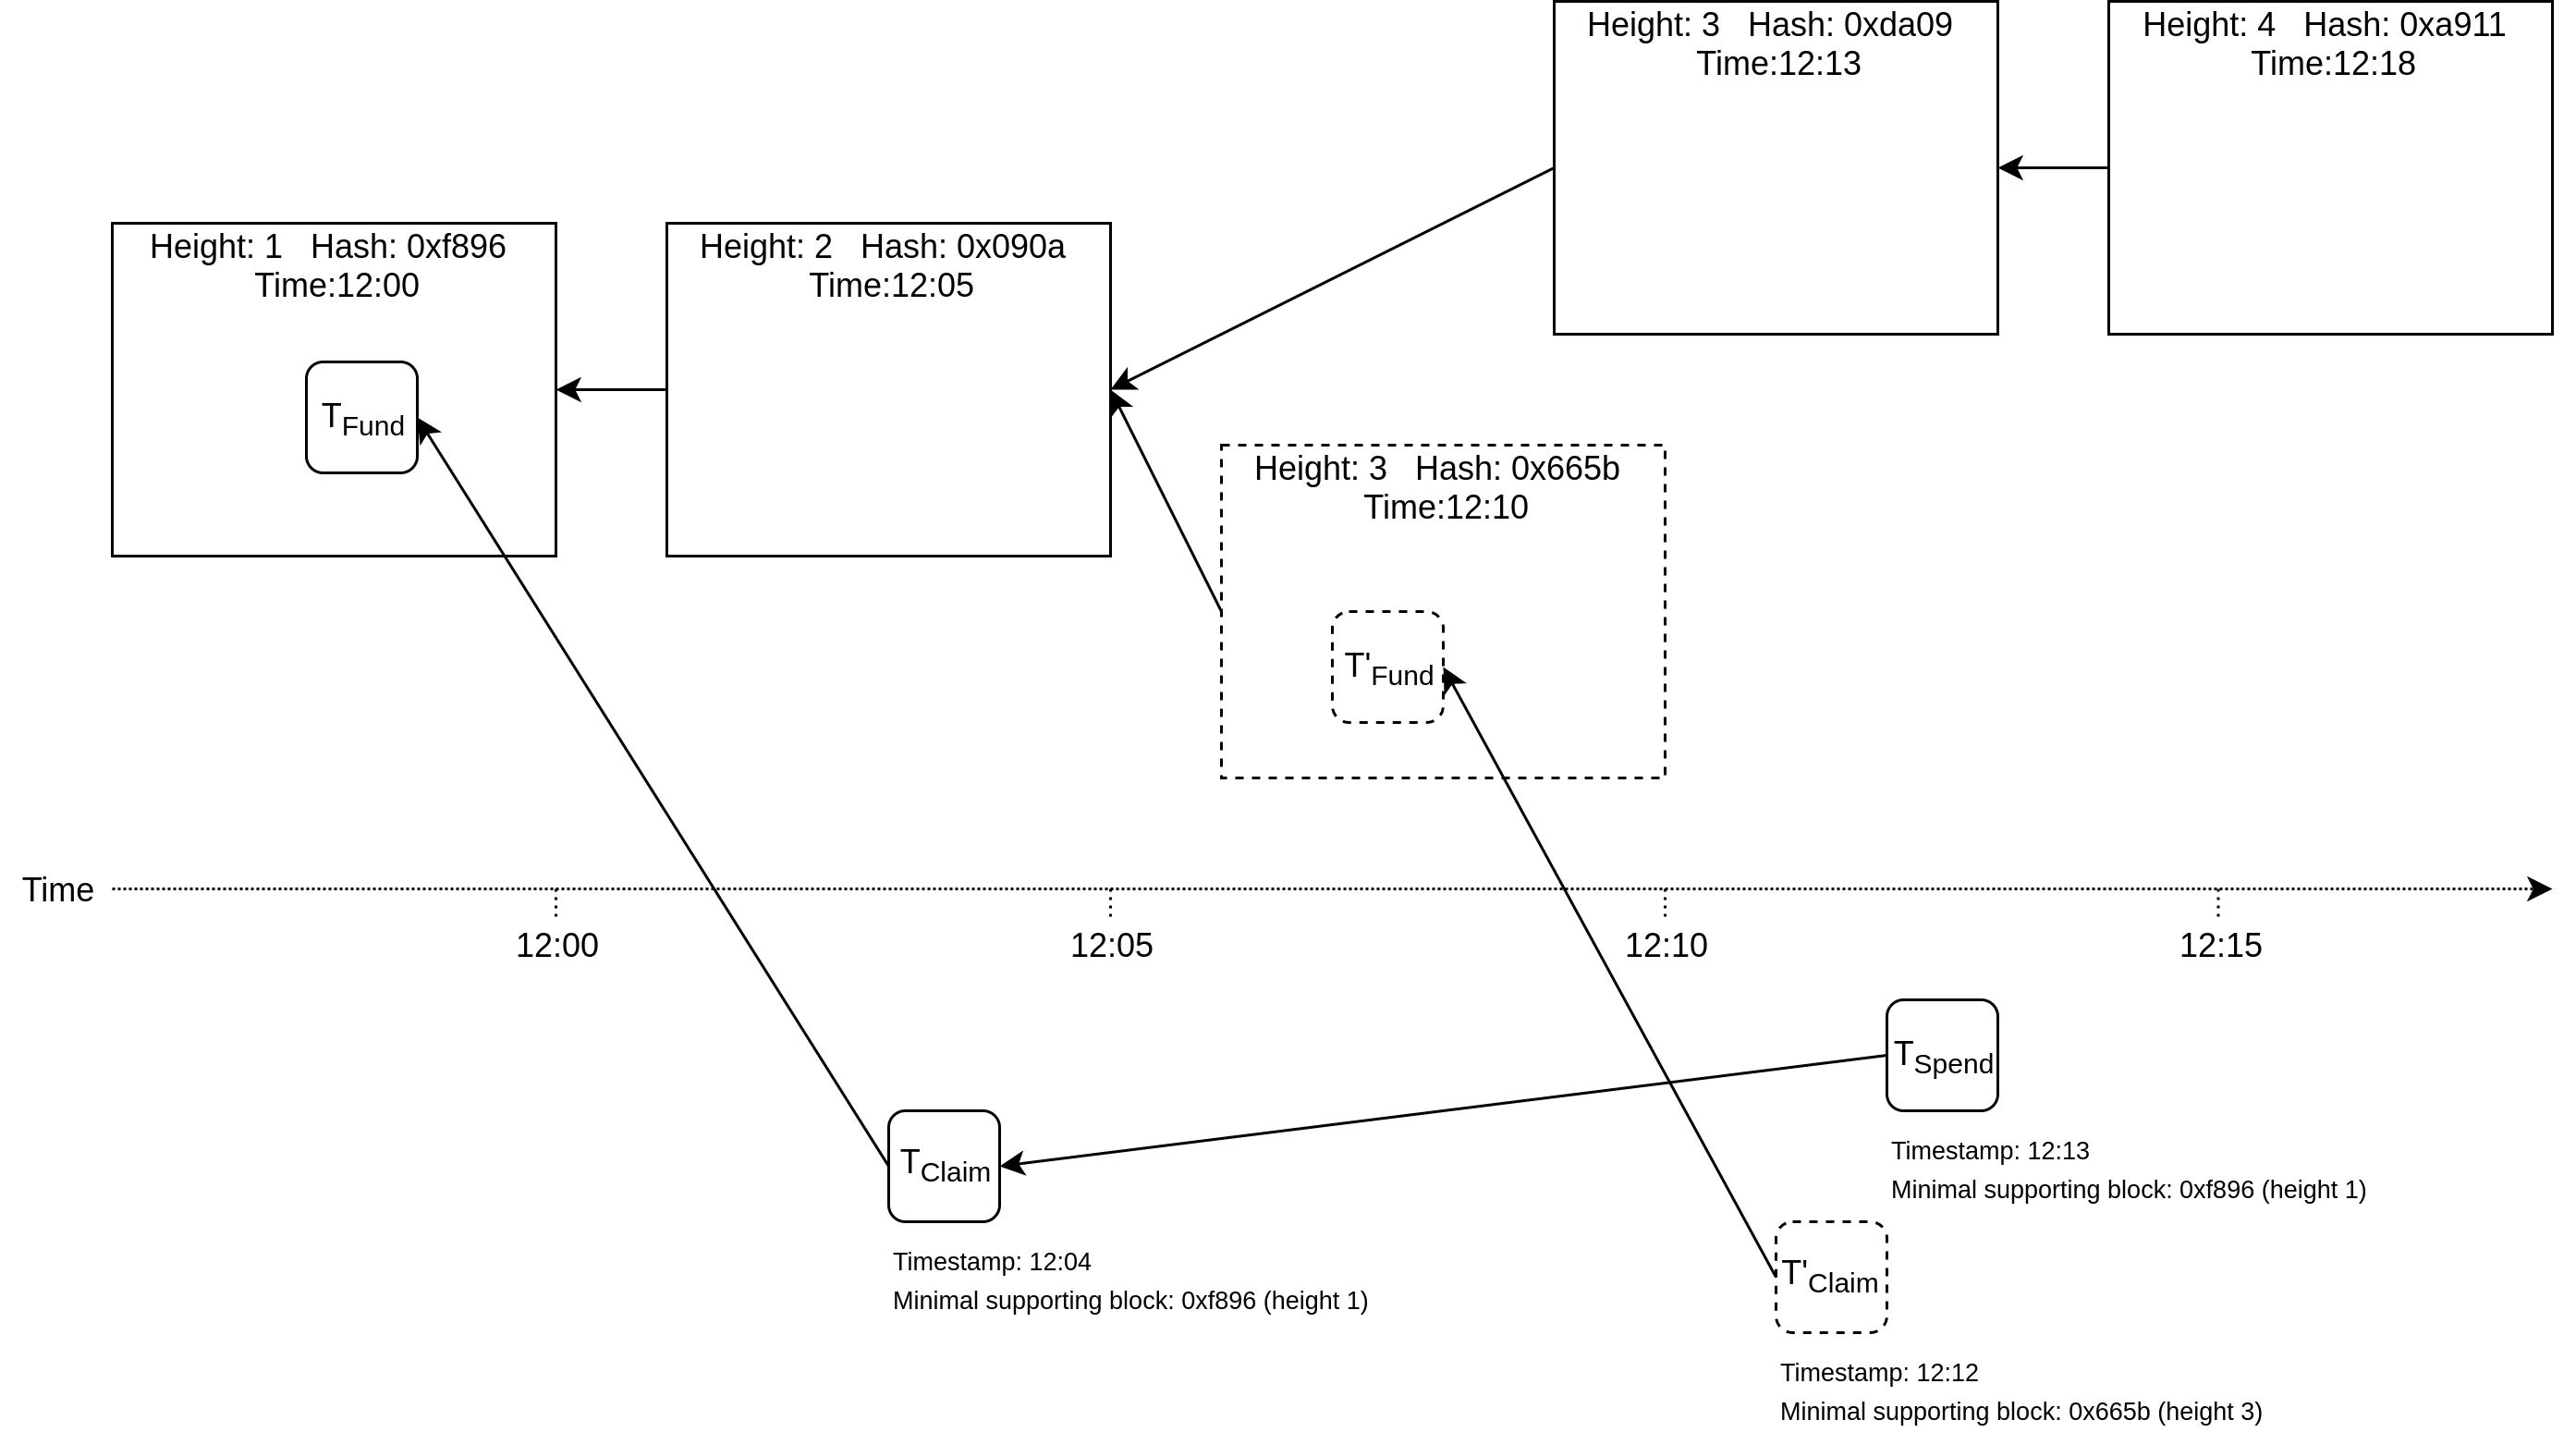
\includegraphics[width=350pt]{img/base-chain-tracking.png}
				\end{center}
				\caption{Base Chain Tracking}
				\label{fig:baseChainTracking}
			\end{figure}
			
			When a Conclave block, $B$ is being constructed, the minimal supporting blocks \index{Minimal supporting block} of all its parent transactions, $P_{i}$, are checked, and $B$'s MSB is set to the highest of those. If there is a base-chain reorganization at block $h$, this will trigger a reorganization on the Conclave chain too. Any Conclave block who's MSB points at a block who's height is $< h$ is guaranteed to be not to be affected and can be kept. Any other blocks must be removed. \\
			
			Were the MSB not present, it would be expensive to figure out which blocks are affected by the re-organization, as it would involve tracing every possible path from the transaction under examination, searching for an claim transaction whose funding outpoint was mined in a block with height $\ge h$.
			
		\subsection{Handling Chain Splits/Reorganizations} 
		A chain split \index{Chain split} \index{Reorganization, chain} happens on the base chain when two different blocks are mined at height $h$. This results in a situation where half the network mines on top of the first block and the other half mines \index{Mining} on top of the second block. Chain splits usually get resolved as soon as block $h+1$ is found, at which point the entire network begins mining on top of block $h+1$, leaving an orphan block \index{Orphan block} at height $h$. Figure \ref{fig:ucSplit1} shows a situation where two bitcoin blocks have been mined at height 1: $1a$ and $1b$. Block $1a$ contains Conclave entry transactions $C1$ and $C2$ and block $1b$ contains Conclave entry transactions $C1$ and $C3$. After blocks $1a$ and $1b$ are mined, 4 more Conclave transactions: $C4$, $C5$, $C6$, and $C7$ appear. \\
		
		$C4$ depends on $C1$ which appears in both blocks $1a$ and $1b$, so no matter which of $1a$ or $1b$ wins, $C1$ will survive, thus $C4$ will also survive. However it's unclear whether $C1$ will historically end up being a member of block $1a$ or block $1b$. Each Conclave block contains the block hash of the most recently mined bitcoin block. Since there are two such blocks with different block hashes, and it's unclear which one will survive, $C4$'s block will get a special block hash which is a combination of both, with each even byte from block $1a$'s hash and each odd byte from block $1b$'s hash. This means more transactions can be built on top of $C4$ since its ancestor, $C1$ is guaranteed to survive. $C4$ is a \textit{definite transaction}.\\
		
		Transactions $C5$ and $C6$ both depend on $C1$ but also on $C2$ and $C3$ respectively. Only one of block $1a$ or block $1b$ will survive, thus one of $C2$ or $C3$ will survive, but we don't yet know which one. $C2$ and $C3$ are \textit{tentative transactions}, \index{Tentative transaction} as are $C5$ and $C6$. Until Bitcoin block 2 is mined, $C5$, $C6$, and any transactions which depend on them, are put on hold, and may not be added to the Conclave blockchain. If they already were added, for example if block $1a$ appeared 1 minute before block $1b$ appeared, they are removed and a Conclave chain re-organization \index{Reorganization, chain} will happen. Any transaction which depends on a tentative transaction is itself a tentative transaction, and may not have any children until it becomes clear if they are on the surviving chain. Two tentative transactions may conflict with other, but not with a definite transaction.\\
		
		Transaction $C7$ is shown for illustration purposes only. The creator of transaction $C7$ knows that there are two competing blocks at height 1, and only one of them will survive, thus its impossible that both $C2$ and $C3$ will survive. This makes $C7$ an \textit{impossible transaction}. \index{Impossible Transaction} Participants should not create such transactions.
		
		
			\begin{figure}[H]
				\begin{center}
					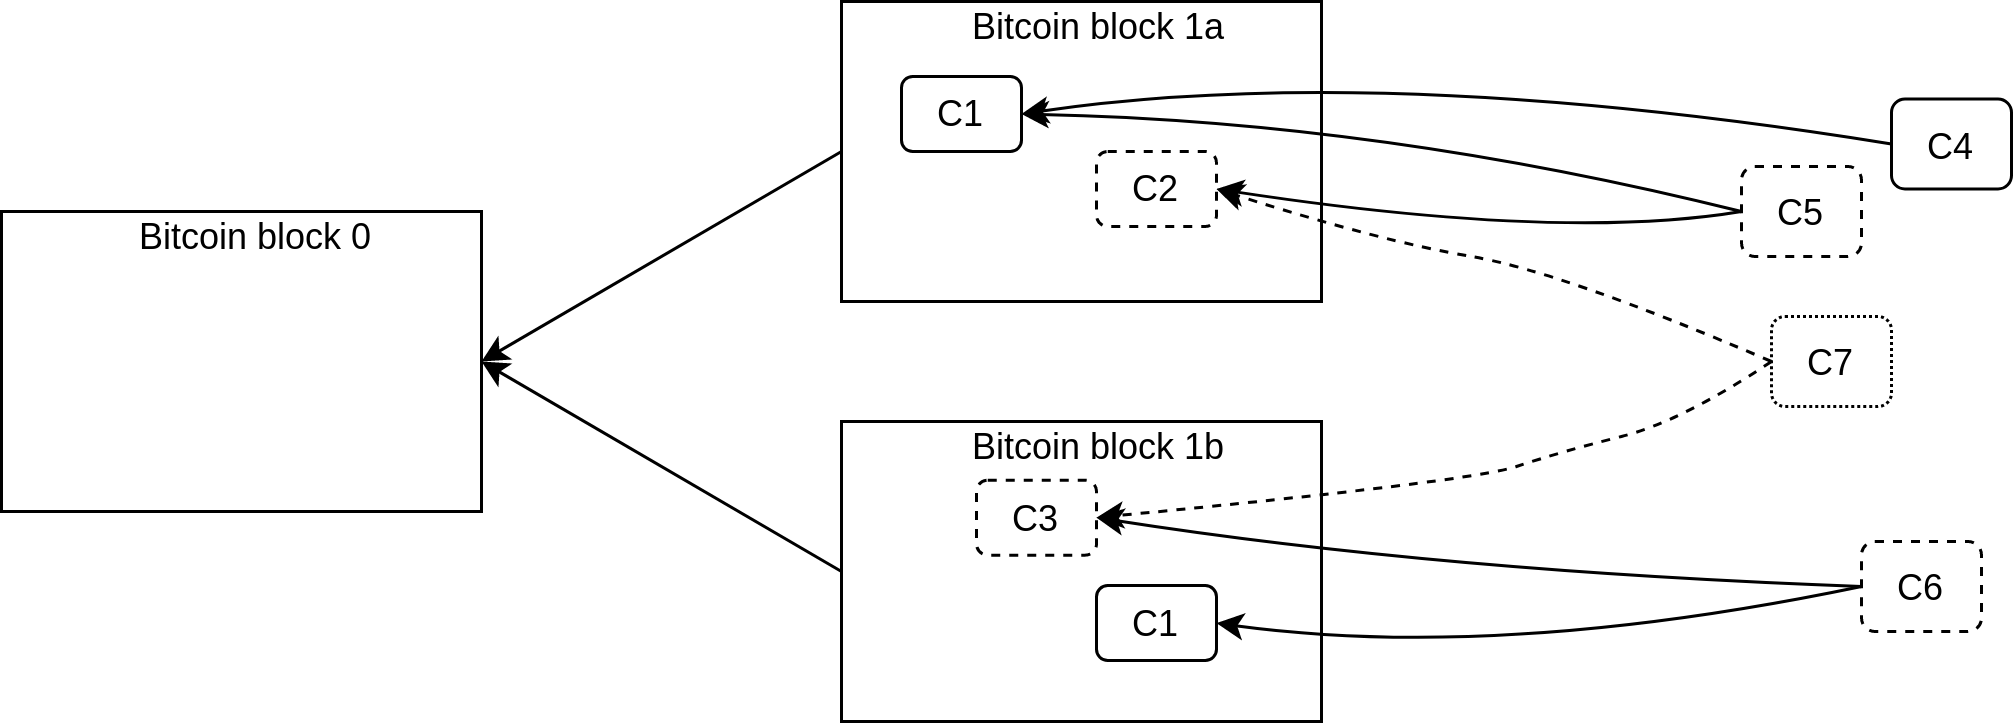
\includegraphics[width=350pt]{img/Chain-Split-1.png}
				\end{center}
				\caption{Unresolved Chain Split}
				\label{fig:ucSplit1}
			\end{figure}
			
			\begin{figure}[H]
				\begin{center}
					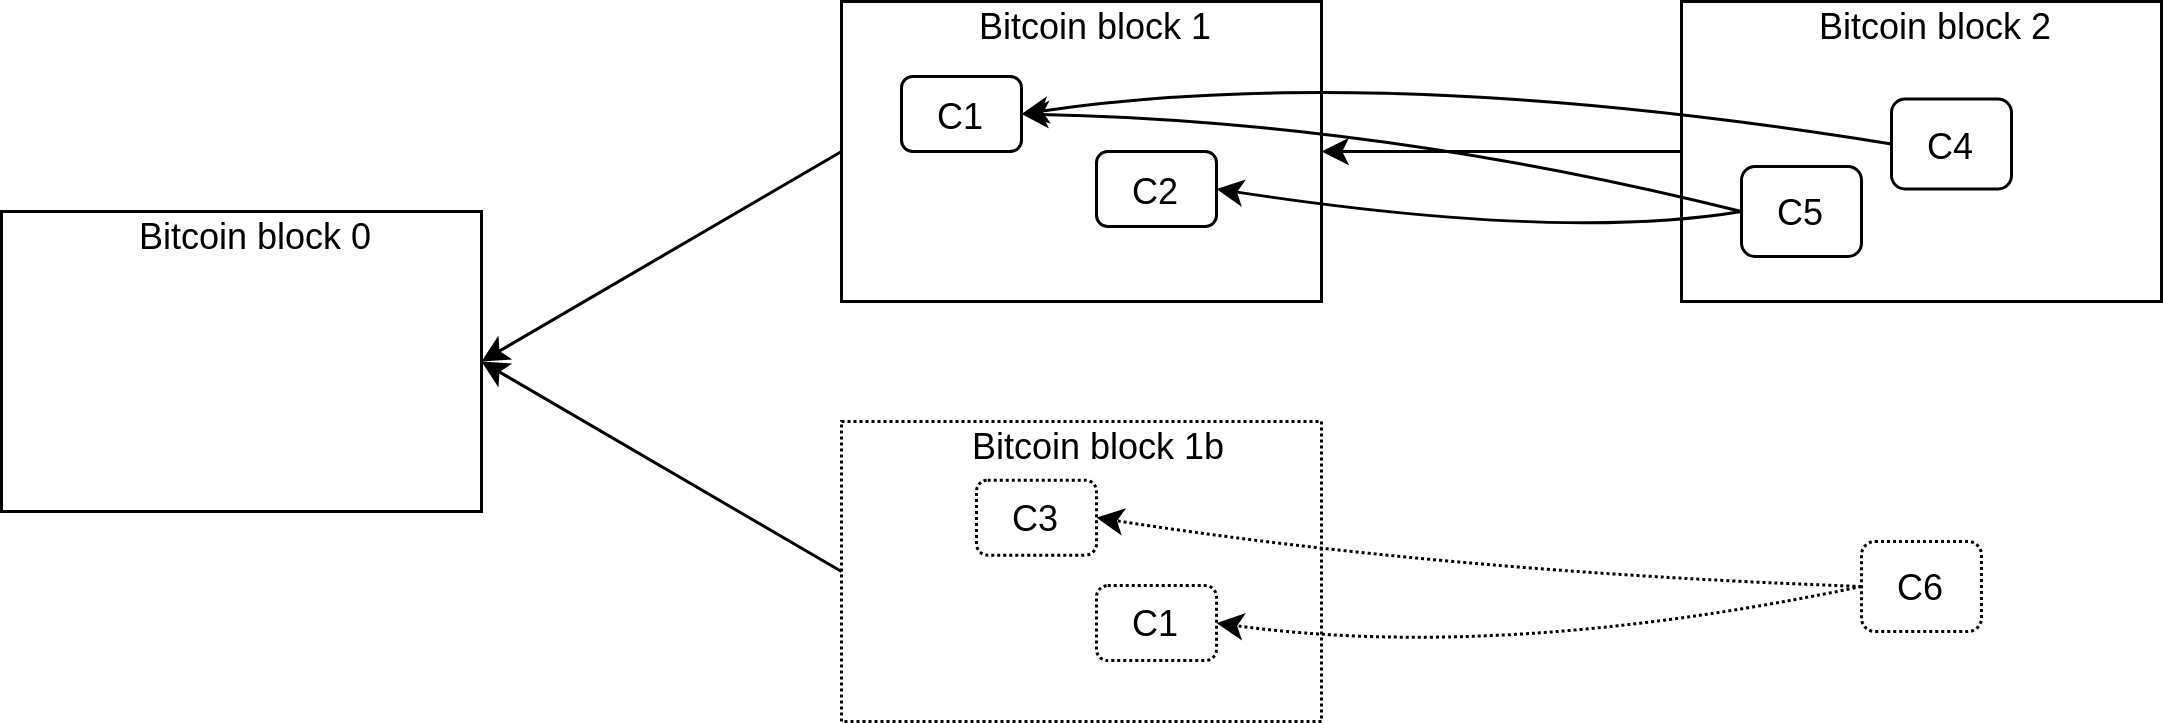
\includegraphics[width=350pt]{img/Chain-Split-2.png}
				\end{center}
				\caption{Resolved Chain Split - Block 1a wins}
				\label{fig:ucSplit2}
			\end{figure}
		
			\begin{figure}[H]
				\begin{center}
					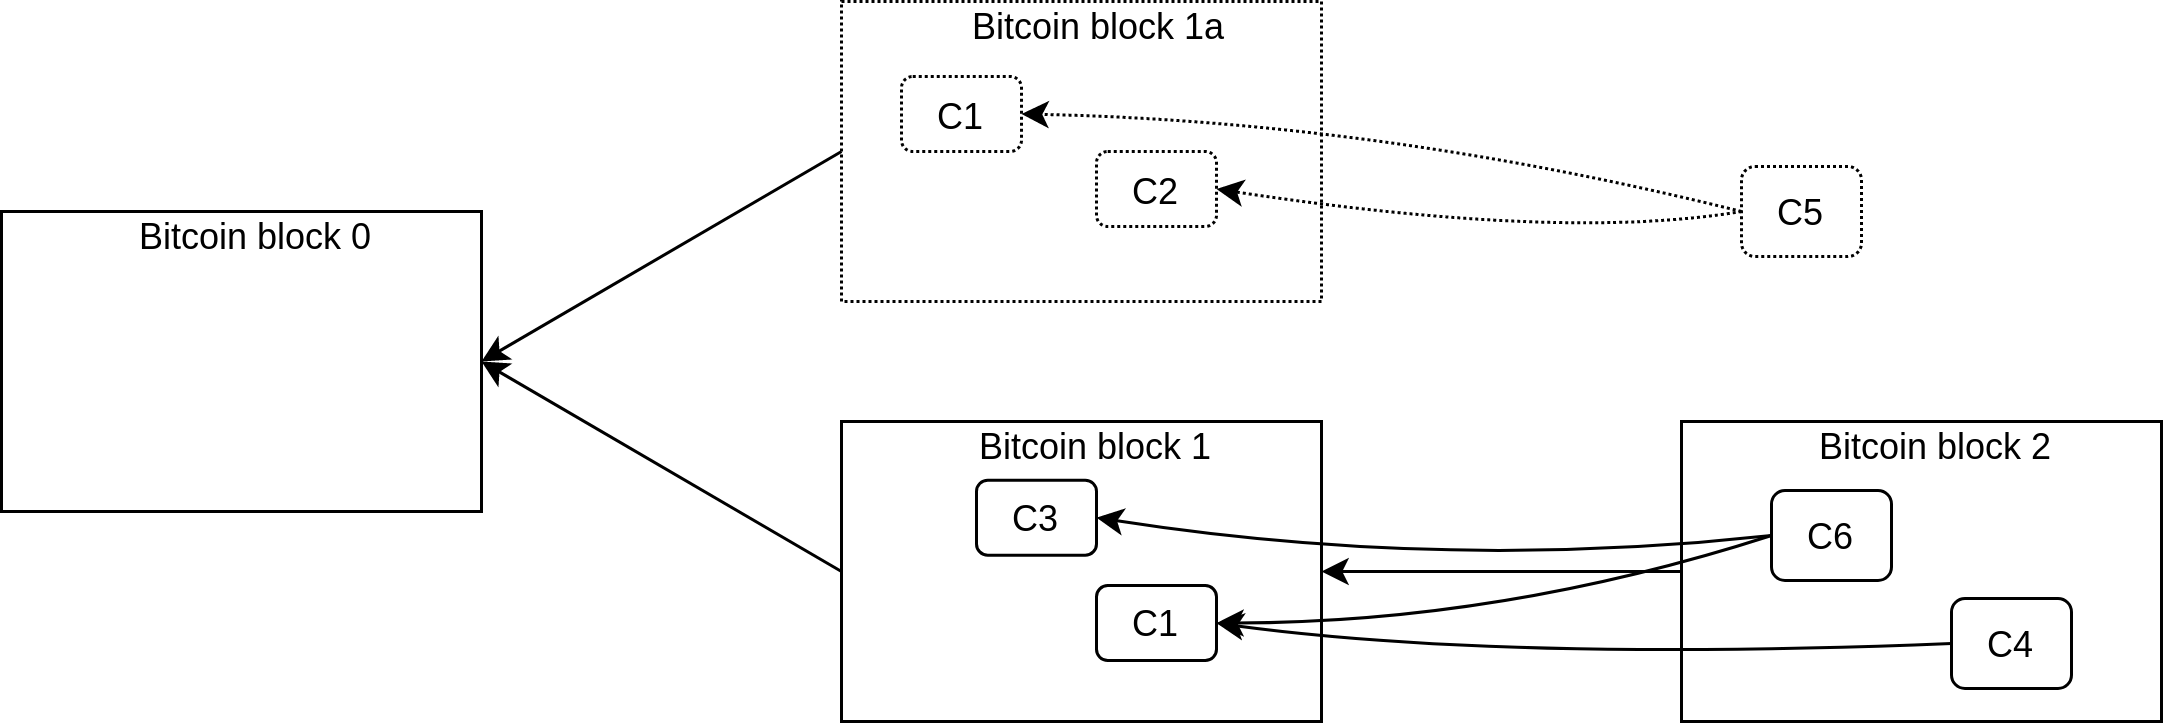
\includegraphics[width=350pt]{img/Chain-Split-3.png}
				\end{center}
				\caption{Resolved Chain Split - Block 1b wins}
				\label{fig:ucSplit3}
			\end{figure}
		
		
		\subsection{Colluding Signers Attack}
			A \textit{colluding signers attack} (CSA) is an attack where trustees entrusted to a UTXO collude and spend the UTXO against the rules of the Conclave protocol. \\
			 
			If a user deposits a large amount of bitcoin to the Conclave network, that bitcoin is stored in a m-of-n multi-signature \index{Multisignature} output, $O$, on the Bitcoin chain. Spending $O$ requires that any $m$ of $O$'s $n$ trustees sign the spend. Ordinarily they will only do this within the rules of the protocol, however $m$ trustees could collude to sign a transaction which spends $O$ outside of the protocol. If this were to happen, the colluders would immediately lose all their trust points, \index{Trust points} and never again be selected as trustees or get paid for signings, meaning they never again earn money as trustees. \\
			
			For such an attack to be financially attractive to a potential colluder, \index{Collusion} the payoff would need to be greater than the amount of money they could make in a reasonable amount of time as an honest participant. Of course, ``a reasonable amount of time" could vary wildly depending on the participant and the amount of money involved. A hard-up participant may need cash as soon as possible and sacrifice long-term income for an immediate payout whereas more financially disciplined participants might not be so tempted, preferring a steady, stable income. \\
			
			If the potential payoff is extremely large, say \$1B, a participant may always prefer the idea of colluding and getting the money immediately, even if they were on track to make that much in a ``reasonable amount of time". \\
			
			When a user wants to deposit money to Conclave, we need an algorithm for choosing the set of $n$ trustees, and $m$, that minimises the probability of a CSA occurring but does not make the spend condition so stringent that the UTXO becomes locked. \\
			
			Let $P$ be a set of 10 Conclave participants with non-zero trust scores:
			\[P = \{Alice, Bob, Carol, Dave, Ed, Fiach, Ger, Hannah, Ian, Jane\}\]

			$P$'s trust scores are:
			
			\[(Alice \rightarrow 77, Bob \rightarrow 55, Carol \rightarrow 29, Dave \rightarrow 21, Ed \rightarrow 15, Fiach \rightarrow 10, Ger \rightarrow 9, Hannah \rightarrow 7,\]
			\[Ian \rightarrow 6, Jane \rightarrow 5)\]
			
			A participant's daily earnings are proportional to their trust score. Suppose each member of $P$ earns $100s$ per trust point per day, then their daily earnings are:
			
			\[(Alice \rightarrow 7,700s, Bob \rightarrow 5,500s, Carol \rightarrow 2,900s, Dave \rightarrow 2,100s, Ed \rightarrow 1,500s, Fiach \rightarrow 1,000s,\]
			\[Ger \rightarrow 900s, Hannah \rightarrow 700s, Ian \rightarrow 600s, Jane \rightarrow 500s)\]
			
			Now, Suppose a Conclave end-user, Isabelle, wants to deposit $20,000s$ to the network. Alice earns $7,700s$ per day so it would take her approximately $2.6$ days to earn $20,000s$. If Alice was designated as being the sole trustee of Isabelle's deposit, it's reasonable to think that Alice would not steal it since it would only take her $2.6$ days to make that amount and would continue to earn money afterwards, whereas if she stole Isabelle's $20,000s$ immediately, she would get $20,000s$ but forfeit all future earnings. \\
			
			Jane, on the other hand might be more tempted to steal the $20,000s$ if given this opportunity since it would take her 40 days to make that amount, and the opportunity to get it immediately despite forfeiting all future earnings might outweigh the choice of earning it honestly over 40 days. \\
			
			But if Jane could earn the $20,000s$ in $20$ days, would she make the same choice? What about $10$ days? Similarly, would Alice still behave honestly if the amount of time it took her to earn $20,000s$ was increased from $2.6$ days to $260$ days? At what point does it become more attractive to behave honestly than dishonestly, \index{Earning} \index{Dishonesty} and vice-versa? Given a deposit amount $D$ and a network participant $p$ we define $eq_p(D)$ as the \textit{equilibrium point} at which $p$ is equally motivated to make $D$ from behaving honestly as from behaving dishonestly.
			
			Going back to Isabelle's deposit, we calculate $eq_{Avg}(20,000)$ to be $3.0$ days meaning 3 days is the average time potential trustees are willing to work honestly in order to earn $20,000s$. Next we calculate how much each participant makes in the equilibrium period by multiplying $3$ by each member of $P$'s daily earnings:
			
			\[(Alice \rightarrow 23,100s, Bob \rightarrow 16,500s, Carol \rightarrow 8,700s, Dave \rightarrow 6,300s, Ed \rightarrow 4,500s, Fiach \rightarrow 3,000s,\]
			\[Ger \rightarrow 2,700s, Hannah \rightarrow 2,100s, Ian \rightarrow 1,800s, Jane \rightarrow 1,500s)\]
			
			Alice makes $23,100s$ in the equilibrium period which is $3,100$ more than she would make if she was to steal Isabelle's $20,000s$ immediately if made the sole trustee, so it's reasonable to expect that she will behave honestly; however all the others make less than $20,000s$ in this period and consequently may try to steal Isabelle's deposit. \\
			
			If we construct the power-set $\mathcal{P}$(P), we can partition its $2^{|P|}$ elements into 2 subsets:
			\begin{enumerate}
				\item Viable trustee sets \index{Viable trustee set}
				\item Non-viable trustee sets \index{Non-Viable trustee set}
			\end{enumerate}
			
			A viable trustee set is any subset of $P$ such that the sum of the earnings of its members during the equilibrium period \index{Equilibrium period} exceeds $D$. In our example, the following sets are viable trustee sets:
			
			\[ \{ Alice \} \mbox{  } \dots \mbox{ because } 23,100s > 20,000s \]
			\[ \{ Bob, Ed \} \mbox{  } \dots \mbox{ because } (16,500s + 4,500s) > 20,000s \]
			\[ \{ Carol, Ed, Fiach, Hannah, Ian \} \mbox{  } \dots \mbox{ because } (8,700s + 4,500s + 3,000s + 2,100s + 1,800s) > 20,000s \]
			\[ P \mbox{  } \dots \mbox{ because } 70,200s > 20,000s \]
			
			Our task is to choose $n$ trustees from $P$, and $m$. If we set $n = |P|$ and include all $10$ participants as trustees, \index{Trustee} our task is simply to find $m$. Since non-viable trustee sets exist with 1 member - for example $\{Jane\}$, $m$ cannot be $1$. $m$ also cannot be $2$ because non-viable trustee sets with $2$ members also exist - for example $\{ Hannah, Ian\}$. If we order $P$ in ascending order of $e_{eq}$, and construct a new set $Q$ by continuing to add participants until the sum of the $e_{eq}$'s of $Q$'s members exceeds $D$, $Q$ will be the minimal safe set comprised of the least-safe members, and we set $m = |Q|$. \\
			
			Carrying out this procedure on $P$, we begin by sorting its members by $e_{eq}$:
			
			\[(Jane \rightarrow 1,500s, Ian \rightarrow 1,800s, Hannah \rightarrow 2,100s, Ger \rightarrow 2,700s, Fiach \rightarrow 3,000s, Ed \rightarrow 4,500s,\]
			\[Dave \rightarrow 6,300s, Carol \rightarrow 8,700s, Bob \rightarrow 16,500s, Alice \rightarrow 23,100s)\]
			
			We construct an empty set $Q = \{\}$ and begin adding members of $P$, starting with Jane, until the sum of the $Q$'s members' $e_{eq}$'s exceeds $20,000s$:
			
			\[ Q = \{  \} \mbox{  } \dots \mbox{ not enough because } 0s < 20,000s \]
			\[ Q = \{ Jane \} \mbox{  } \dots \mbox{ not enough because } 1,500s < 20,000s \]
			\[ Q = \{ Jane, Ian \} \mbox{  } \dots \mbox{ not enough because } 3,300s < 20,000s \]
			\[ Q = \{ Jane, Ian, Hannah \} \mbox{  } \dots \mbox{ not enough because } 5,400s < 20,000s \]
			\[ Q = \{ Jane, Ian, Hannah, Ger \} \mbox{  } \dots \mbox{ not enough because } 8,100s < 20,000s \]
			\[ Q = \{ Jane, Ian, Hannah, Ger, Fiach \} \mbox{  } \dots \mbox{ not enough because } 11,100s < 20,000s \]
			\[ Q = \{ Jane, Ian, Hannah, Ger, Fiach, Ed \} \mbox{  } \dots \mbox{ not enough because } 14,600s < 20,000s \]
			\[ Q = \{ Jane, Ian, Hannah, Ger, Fiach, Ed, Dave \} \mbox{  } \dots \mbox{ enough because } 20,900s > 20,000s \]
			
			Thus $m = |Q| = 8$ and Isabelle's deposit of $20,000s$ will be encumbered in an 8-of-10 multisignature with all members of $P$ as trustees. \\
			
			Since $Q$ contains the $m$ weakest members of $P$, no weaker subset of size $m$ or greater can exist. If we removed Dave from $Q$, reverting back to the second-last step, we could distribute the $20,000s$ among Jane, Ian, Hannah, Ger, Fiach and Ed such that each of them receive an amount greater than what they would earn in $eq_{Avg}(20,000)$, and may be tempted to collude. \\
			
			\subsubsection{Choosing $n$}
			
			In the previous example, I set $n$ to the maximum possible value, $10$. If block space is unlimited, increasing $n$ to be as high as possible increases the pool of potential signers so should always be done, however in the real world, block space is limited. Suppose we were limited to 5 trustees per transaction. In this case we would remove the 5 smallest members of $P$, meaning $P$ and its members' $e_{eq}$'s would be:
			
			\[(Ed \rightarrow 4,500s, Dave \rightarrow 6,300s, Carol \rightarrow 8,700s, Bob \rightarrow 16,500s, Alice \rightarrow 23,100s)\]
			
			Therefore $Q$ would be $\{Ed, Dave, Carol\}$, making it a 3-of-6 multisignature. \index{Multisignature}
			
	\section{Low Level}
		In this section I discuss some of the low-level ``building blocks" of Conclave: the cryptographic primitives, the common data structures, and the reasoning behind their design, and some of their implementation details.
		\subsection{Node IDs And Keys}
			Every node on the Conclave network has a public/private keypair which it uses for digital signatures and asymmetric encryption operations. Each node also has a unique ID, although this ID is nothing but the node's public key. I may use the term \textit{node ID} or \textit{public key} depending on context, but refer to the same thing. No two nodes can have the same node ID. If they do, then they are the same node, and therefore must have the same public/private keypair. An example of a node ID \index{Node ID} is:
		\begin{center}
		  \texttt{024c09a24e80c80b47341a4608e371194982bad858eb25201e1b941d012004bc2b}
		\end{center}
		
		\subsection{Cryptography}
		Conclave uses the same type of asymmetric cryptography as Bitcoin: elliptic curve cryptography with the Secp256k1 \cite{secp256k1} curve. There are several reasons for going with this choice:
		  \begin{enumerate}
		  	\item Security - this curve has been in production on the Bitcoin network and several other cryptocurrencies for over 10 years and has not been shown to be compromised
		  	\item Interoperability - using the same curve as the base chain means a given private key will generate the same public key, and therefore the same public key hash, meaning a classic bitcoin address can trivially be converted to a Conclave address and vice-versa \index{Elliptic curve cryptography}
		    \item Convenience - existing wallets and client software which already interacts with Bitcoin will likely already have the Secp256k1 functions available and not require any additional dependencies 
		  \end{enumerate}
		\subsection{Hash Functions}
		Conclave also uses the same hash functions as Bitcoin: SHA256 and RIPMD160, and uses them in a similar way: RIPEMD160 $\circ$ SHA256 for hashing public keys to make addresses, and SHA256$^2$ for hashing transactions, blocks, and everything else. \\
		
		Again, the reasoning behind this decision is the same as with the EC cryptography: These hashing functions have been in production for over 10 years and not shown any weakness. Finding any SHA-256 collision with 50\% probability requires computing approximately $4 \times 10^{38}$ \cite{bday} hashes. In 2020, Bitcoin's mainnet hash rate is approximately 100 exahashes/second. \index{Hash collision} \\
		
		This means that to find a single SHA256 collision using the hashing power of the entire Bitcoin network with 50\% probability it would take:
		\begin{center}
		$\frac{4 \times 10^{38} Hashes}{100 \times 10^{18} Hashes/second} = 4 \times 10^{18} seconds$
		\end{center}
		which is over 126,839,167,935 years, and that is to find \textit{any} hash collision, which is almost certainly, if found, not going to facilitate the stealing of bitcoin. In addition, such an attack would require enough storage space to store the $4 \times 10^{38}$ previously attempted hashes. Since each hash is 32 bytes, a total of 10,587,911,840,678,754 \textit{yobibytes} \cite{yobibyte} \index{Yobibyte} of storage space would be required.
		
		\subsection{Addresses}
			Currently there are four types of address on the Bitcoin network:
			\tiny
			\begin{center}
				\renewcommand{\arraystretch}{1.9}
				\begin{tabular}{ |p{2cm}|p{4.8cm}|p{7.2cm}| } 
					\hline
					\textbf{Address Type} & \textbf{Description} & \textbf{Example} \\
					\hline
					Pay-to-public-key-hash\newline(P2PKH) & Payments made to P2PKH addresses may be spent with no special conditions aside from possession of the underlying public/private keypair. & 147SwRQdpCfj5p8PnfsXV2SsVVpVcz3aPq \\
					Pay-to-script-hash (P2SH) & Payments made to P2SH addresses may be spent on the condition that the payee possesses the script to which the payment was made, and can satisfy that script. & 3Nb89icKvi6X7c3C2GQYRUkY7Ym6sQtnbH \\
					Pay-to-witness-public-key-hash (P2WPKH) & Payments made to P2PKH addresses may be spent with no special conditions aside from possession of the underlying public/private keypair. & bc1qh5c78mgptx2nzk45xevfk6g8n7vftu880hntfx \\
					Pay-to-witness-script-hash (P2WSH) & Payments made to P2WSH addresses may be spent on the condition that the payee possesses the script to which the payment was made, and can satisfy that script with a witness. & bc1qwqdg6squsna38e46795at95yu9atm8azzmyvckulcc7kytlcckxswvvzej \\
					\hline
				\end{tabular}
			\end{center}
			\normalsize
			Hashed data accounts for the majority of bits in these addresses . The hashes are augmented with some status bits and the result is checksummed and wrapped in a reversible encoding scheme which becomes the address. P2PKH and P2WPKH addresses contain hashes of Secp256k1 public keys, whereas P2SH and P2WSH addresses contain hashes of scripts written in the Bitcoin script language. The status bits indicate (among other things):
			\begin{enumerate}
				\item What type of thing the hash is \textit{of} (public key or script)
				\item What network the address belongs to (Bitcoin, Litecoin, Dash, etc.)
				\item If it is a mainnet or testnet address
			\end{enumerate}
			P2PKH addresses have been part of the Bitcoin protocol since the beginning and still account for the vast majority of addresses. They represent the payee as the possessor of a Secp256k1 private key, who may spend funds sent to the address, so long as they possess that private key. P2SH addresses were introduced in 2012 with BIP 16 \cite{p2sh} soft fork \index{Soft Fork} \index{BIP-16} and represent the payee as the possessor of a script who must also be able to satisfy that script by ensuring certain conditions are true such as spending after a certain date, and usually also the possession of a private key or keys. \\

			P2PKH and P2SH addresses, which I will refer to as ``classic" addresses, use a crude checksumming scheme which involves making a double-SHA256 hash of \texttt{(prefix | hash)} where prefix contains all the status bits, then chopping off the first 4 bytes of that hash which is used as the checksum, and finally base58-encoding \texttt{(prefix | hash | checksum)} to make the address. \\
			 
			P2WPKH and P2WSH addresses, which I will refer to as ``segwit" addresses, use more advanced checksumming and encoding techniques \cite{bech32}, and funds sent to them result in smaller and thus cheaper transactions for the payee \cite{segwit}, since the signature or ``witness" data is moved off the blockchain.

			A Conclave user can send Bitcoin to, and receive Bitcoin from, any of these four types of addresses without any knowledge or interaction from the payee. This is an important improvement over LN which requires the payee to first send an invoice to the payer requesting payment, then the payer must promptly pay the invoice while the payee is still online.
			\subsubsection{Conclave Addresses}
			Conclave addresses have more in common with classic addresses than segwit addresses. \index{Address, segwit} They are encoded using the same base58 \index{Base58} alphabet as classic addresses, therefore they look more similar to them than to the longer, base32 segwit format. As with classic and segwit addresses, Conclave addresses are mainly comprised of a hash, along with some status bits and a checksum. At present, we define two types of mainnet Conclave address, which can pay to either a public key or to a script:
			\tiny
			\begin{center}
				\renewcommand{\arraystretch}{1.9}
				\begin{tabular}{ |p{2cm}|p{4.8cm}|p{7.2cm}| } 
					\hline
					\textbf{Address Type} & \textbf{Description} & \textbf{Example} \\
					\hline
					Pay-to-conclave-public-key-hash\newline(P2CPKH) & Payments made to P2CPKH addresses may be spent with no special conditions aside from possession of the underlying public/private keypair. & 5Xjy8xUQZpdnvzhLJmJktWjMwZ9hLHPG \\
					Pay-to-conclave-script-hash (P2CSH) & Payments made to P2CSH addresses may be spent on the condition that the payee possesses the script to which the payment was made, and can satisfy that script. & 4YEsF1a9naovExb6zYsWtPxH5Lt6BHJi \\
					\hline
				\end{tabular}
			\end{center}
			\normalsize

			Like classic addresses, Conclave addresses use RIPEMD160 $\circ$ SHA256 \index{RIPEMD} \index{SHA256} as the hashing scheme, regardless of whether the thing being hashed is a public key or a script, but use less bits for the checksum and network identification, and have less redundant bits. This results in a slightly shorter address. As can be seen from Figure \ref{fig:addressBitmap}, the first bit indicates whether it is a mainnet or testnet address, the next 3 bits denote the address class giving 8 possible classes, 2 of which are so far defined: P2CPKH and P2CSH, followed by 20 checksum bits and finally the 160-bit hash, making a total length of 184 bits, meaning a Conclave address is 16 bits shorter than a classic address. 

				\begin{figure}[H]
					\begin{center}
					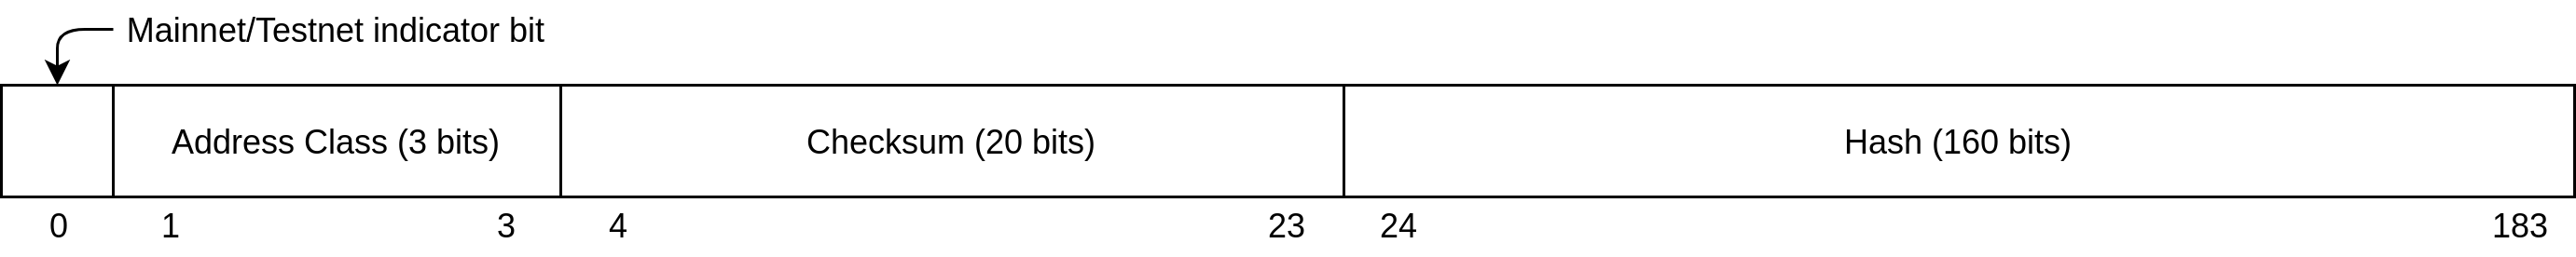
\includegraphics[width=400pt]{img/conclave_address.png}
					\end{center}
					\caption{Bit-map of Conclave Address}
					\label{fig:addressBitmap}
				\end{figure}

			The checksum algorithm consists of a simple modular arithmetic operation. The first 4 bits are appended to the hash, converted to a 164 bit integer, and reduced modulo $2^{20}-3$, which is the largest prime which fits into 20 bits. A prime modulus guarantees that any single bit-flip in the 164-bit integer, or single character error in the base58 representation will produce a different checksum.
			Flipping a bit is the same as either adding or subtracting a power of two. \index{Power of two} If that power of two is less than $2^{20}$, the checksum will be different regardless of whether the modulus is prime, but if the power of two is $2^{20}$ or greater, the only way the checksum can remain the same is if the modulus is a factor of the power of two, but no power of two has any prime factors other than 2, so the checksum will change if there is a single bit-flip. \index{Checksum} Bit-flips \index{Bit-flip} are almost a non-issue in 2020, since most data is encrypted and protected with mechanisms such as MACs \\	
			
			 If a single base58 character is wrong, a different checksum is guaranteed if it's one of the last 3 characters, since this will cause a deviation no greater than $57 \times 58^2$, which is smaller than the modulus. otherwise an integer of the form $n \times 58^{m} \mid 0 < n < 58, 3 \le m$ is effectively added or subtracted to the 164-bit integer. The only way the checksum can remain the same after this operation is if the modulus is a factor of $n \times 58^{m}$, but the only prime factors \index{Prime factorization} of numbers of this form are 2, 29, and other primes between 3 and 58. The modulus is far higher than any of these numbers, so again the checksum will change. \\
			 
			 If we assume that a person mis-types 1 in every 10 characters, we can calculate the probability of them mis-typing a Conclave address \textit{and} the checksum not changing, resulting in a loss of funds. A Conclave address contains 32 characters. We first compute the probability \index{Probability} of making no mistakes, which is \texttt{binom(32, 32, 0.9)} or $0.0343368382$. Next we consider the probability of making 1 mistake, which is the same as getting 31 characters correct, which is \texttt{binom(31, 32, 0.9)} which is $0.0343368382$, which, as I've shown, is guaranteed to be caught, so may be added to the cumulative total. \\
			 
			 The probability of making 2 mistakes is \texttt{binom(30, 32, 0.9)} or $0.2102601450$, but there is a $1\over{2^{20} - 3}$ chance of the checksum not catching it, meaning there is a $1 - {1\over{2^{20} -3}}$ that it will be caught, which we must take into account, so $0.2102601450$ is multiplied by $1 - {1\over{2^{20} -3}}$, to give the probability of mistyping 2 characters but the error being caught, which is $0.2102599445$. We continue this process of summing the probabilities of the possible events where the result is no loss in funds, and the final probability can be shown to be $0.9999991955$, which is less than 1 per million. \\
			 
			 However in the real world, the probability is likely to be far less than 1 per million, since I've made the bold assumption that the user will never notice if they've made a mistake. In reality, a user will almost surely notice if they make more than 3 typing errors, in which case they are likely to more carefully inspect and type the address, effectively reducing the net probability of a single mis-typed character. \\
			 
			 
			 
		\subsection{Scripts and Transactions}
			Since Conclave is effectively a re-implementation of the Bitcoin protocol on a new blockchain, scripts and transactions are similar. Conclave to Conclave transactions behave in the exact same way as Bitcoin to Bitcoin transactions: both contain \texttt{version} and \texttt{lockTime} fields, a set of inputs and a set of outputs. Each input spends an output in a previous transaction and that spend depends on the concatenation of the input's \texttt{scriptSig} with the output-being-spent's \texttt{scriptPubKey} evaluating to true when run in the script interpreter. Conclave shares Bitcoin's script interpreter and language, and replicates all the consensus rules, therefore not only standard P2PKH and P2SH transactions but all ``special" transaction types such as multisignatures, timelocks, \index{Timelock} crowdfunds, \index{Crowdfund} blank cheques, hash puzzles, coin joins and \texttt{OP\_RETURN} (arbitrary data), are all possible on Conclave. This means Conclave could also be used as a faster, cheaper alternative base layer for the Lightning network.
			\newpage
	\section{Implementation}
		\subsection{The Conclave Dæmon}
			The Conclave Dæmon, \textit{conclaved}, is the primary ``node" software program which is tasked with maintaining the Conclave network. The Conclave network consists of many instances of the dæmon running concurrently and sharing gossip with each other. \\

			\begin{figure}[H]
				\begin{center}
				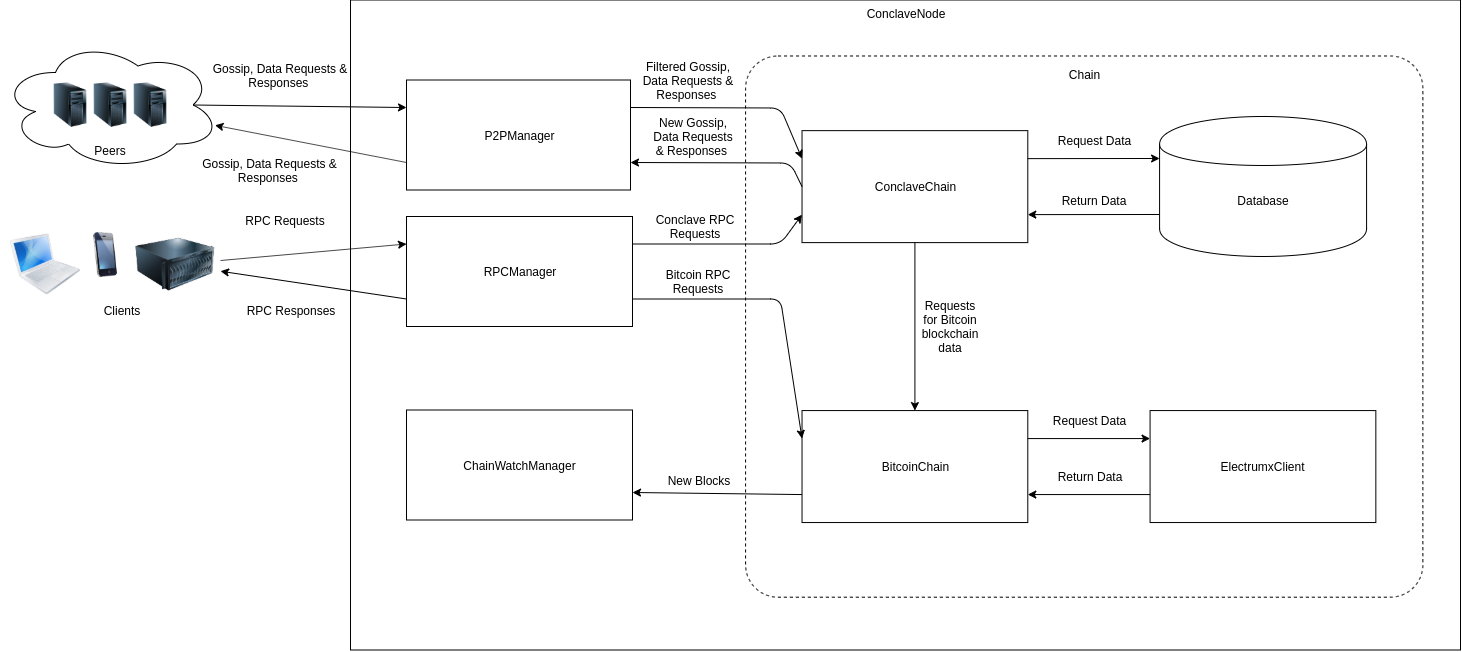
\includegraphics[width=400pt]{img/conclaved.png}
				\end{center}
				\caption{Block diagram of \texttt{conclaved}}
				\label{fig:conclavedBlockDiagram}
			\end{figure}
			
			The dæmon is designed in a modular, object-oriented way, with well-defined dependencies and interfaces, so that components may be upgraded, swapped or stubbed out as quickly as possible with minimal disruption to the network. I will now describe each of the components shown in Figure \ref{fig:conclavedBlockDiagram}.
			\subsubsection{ConclaveNode}
			The \texttt{ConclaveNode} component is the top-level component which contains everything required for one logical node to run. Each \texttt{conclaved} process contains one instance of \texttt{ConclaveNode} which has a configuration including its private key node ID. It's possible for several instances of \texttt{conclaved} to run on different machines with the same configuration, horizontally scaling one logical node across many physical nodes. It's also possible to run several \texttt{ConclaveNode}s on the same machine for experimental purposes. 
			\subsubsection{P2PManager}
			The \texttt{P2PManager} component is responsible for handling the node's interactions with other nodes (peers) on the Conclave network. The \texttt{P2PManager}'s tasks can be broken down into two broad categories: \textit{connection management} and \textit{gossip management}. \\
			
			On bootstrap, the \texttt{P2PManager} will read the set of hard-coded seed nodes' addresses and attempt to make ``first contact" with another node on the network. That initial peer's \texttt{P2PManager} will then send a list of other nodes it knows to be online, and the \texttt{P2PManager} will connect to these too. Over time, the \texttt{P2PManager} attempts to maintain a set of connections such that:
			\begin{enumerate}
			  \item Peers' \texttt{nodeId}s are spread as evenly as possible over the 256-bit keyspace. This maximises the potential amount of data the node has access to in 1 hop, and keeps the overall network structure efficient.
			  \item Trust scores of a node's peers should follow the same distribution as the trust scores of the entire network (excluding zero-trust nodes) This ensures a balanced topology which is not prone to centralization.
			  \item Peers are responsive and respond to pings.
			\end{enumerate}
			The second task of the \texttt{P2PManager} is gossip management. \index{P2P} \index{Gossip} If a new transaction is posted from a user to a node through the \texttt{RPCManager}, \index{RPC} the transaction is passed to the \texttt{P2PManager} for relay, so that the entire network can learn about it. Similarly, if a node's \texttt{ConclaveChain} thinks it has discovered a new block, that block will be passed to the \texttt{P2PManager} for relay to the rest of the network. The same applies to newly endorsed transactions, or emergency system-level state changes such as revoked keys and dishonesty reports. \\
			
			This traffic is known as \textit{gossip} and the \texttt{P2PManager} checks each piece of gossip, verifying its digital signature and ensuring it's not malicious or spam, acting like a firewall/router, ensuring the other components receive gossip they are likely to find useful, and never receive the same gossip twice. Similarly, gossip is never sent or relayed to the same peer twice, unless explicitly requested.
			
			\subsubsection{RPCManager}
			The \texttt{RPCManager} component listens for incoming RPC requests from clients and processes those requests. The \texttt{RPCManager} contains a set of methods, conforming to the JSON-RPC 2.0\cite{jsonrpc2} specification, with each method performing a specific task. The \texttt{RPCManager} interacts with several other components in order to do its job, typically the \texttt{ConclaveNode}, \texttt{BitcoinChain}, and \texttt{ConclaveChain} components. \\
			
			Adding a new RPC method involves creating a \textit{request class}, \textit{handler function}, and \textit{response class}.  The request class contains the arguments to the method, the response class contains the result, and the handler does the job of reading the request and returning the response. Each handler receives a reference to the parent \texttt{ConclaveNode}, which itself contains its sub-components, and queries these components through their public interface. \\
			
			The \texttt{RPCManager} contains two queues: a request queue and response queue, and 3 sub-components which allows it to process RPC requests asynchronously utilizing multiple CPUs. The \texttt{RPCAcceptor} listens for incoming requests, parses them into \texttt{Request} objects, and enqueues them on the request queue. A little while later the request is dequeued by a free \texttt{RPCProcessor} and sent to the appropriate handler, depending on the type of request. When the handler has completed and returns a \texttt{Response}, the \texttt{RPCProcessor} enqueues it on the response queue. A little while later the \texttt{Response} is dequeued by the \texttt{RPCDispatcher} and sent out on the same connection it came in on. \\
			
			Since a handler may take some time to process and each processor can only process one request at a time, a pool of several \texttt{RPCProcessor}s is spun up on startup, each in its own thread. All the \texttt{RPCProcessors} contend to dequeue the next request from the request queue, and a system of mutexes within the queue ensures the request gets dequeued to only one \texttt{RPCProcessor}. Currently there is only one \texttt{RPCAcceptor} and one\texttt{RPCDispatcher} per node since reading and writing sockets is usually not a bottleneck. Each request is tagged by the \texttt{RPCAcceptor} with a pointer to a low-level structure which ultimately contains a reference to the socket on which the request came in on. This pointer ``travels" with the request on to the request queue, and is attached to the response by the \texttt{RPCProcessor} after processing, until the \texttt{RPCDispatcher} finally dequeues the response and writes the response out on the socket and closes it. \\
			
			\begin{figure}[H]
				\begin{center}
				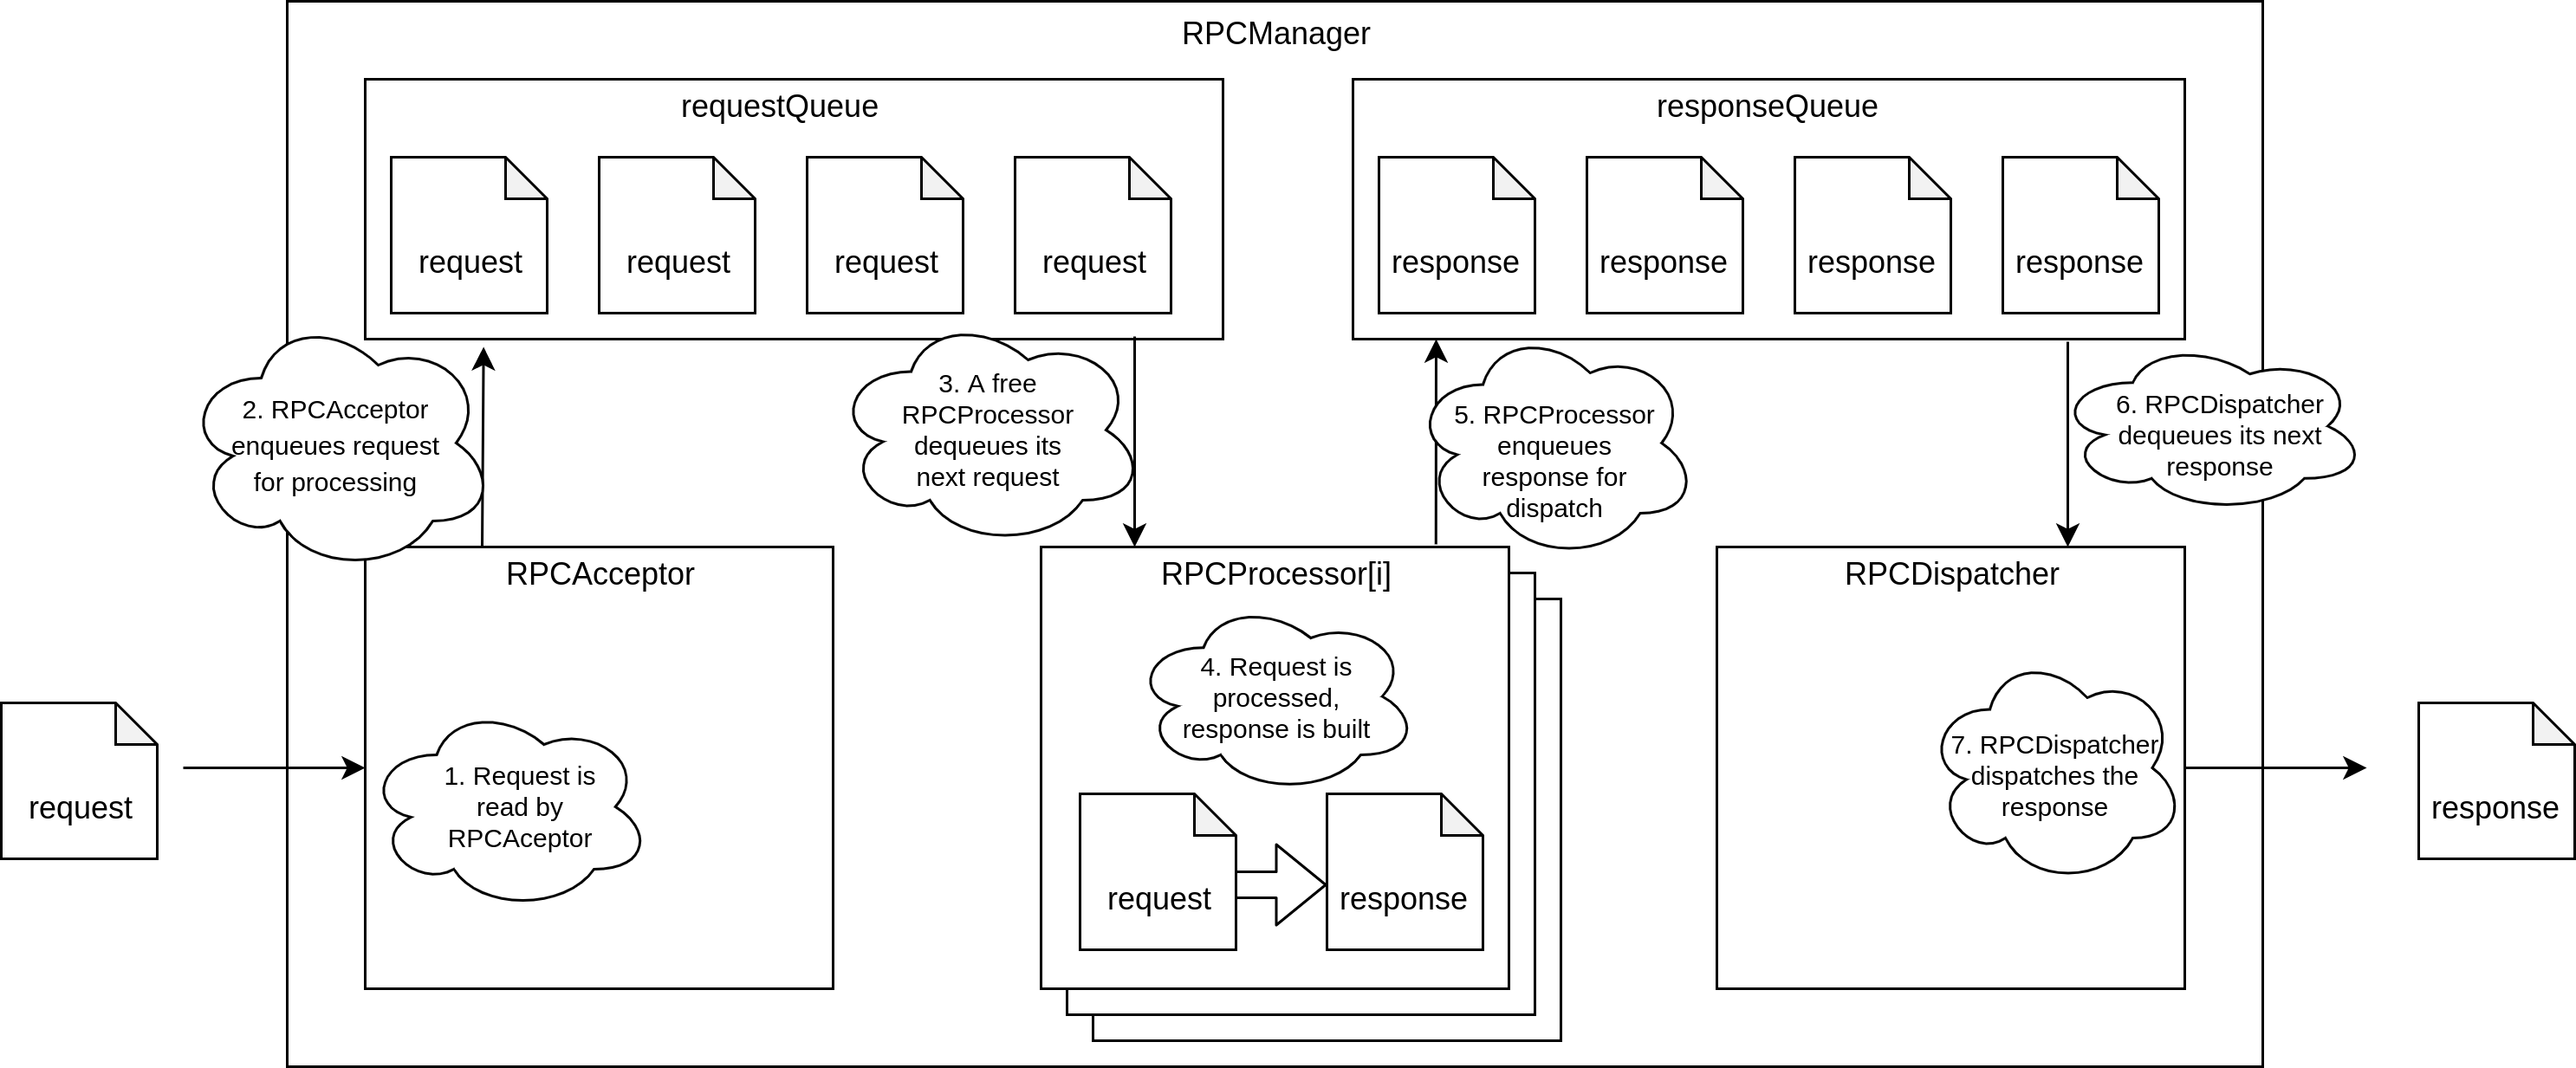
\includegraphics[width=400pt]{img/rpc-queues.png}
				\end{center}
				\caption{\texttt{RPCManager} internals}
				\label{fig:rpcManager}
			\end{figure}
	
			\subsubsection{ChainWatchManager}
			The \texttt{ChainWatchManager} component monitors the Bitcoin blockchain and mempool \index{Mempool} for new transactions which affect Conclave. New transactions are fed to the \texttt{ChainWatchManager} by the \texttt{BitcoinChain} component. When a new block is mined, the \texttt{ChainWatchManager} scans every transaction looking for transactions of interest to Conclave, and when it finds them, takes the relevant actions. The \texttt{ChainWatchManager} needs to check every transaction in every block so keeps a checkpoint on disk of the most recently scanned block and re-scans from that block when the dæmon starts up. \\
			
			The most important task of the \texttt{ChainWatchManager} is looking out for changes to the Conclave system parameters including newly blacklisted nodes. It's important to blacklist nodes as soon as possible after a blacklisting has been authorized through either a self-blacklisting or a community-signed blacklist order so blacklistings are enforced as soon as they are seen in the mempool.
			\subsubsection{BitcoinChain}
			The \texttt{BitcoinChain} component provides an interface to the Bitcoin blockchain, allowing a caller to submit new transactions, and get blockchain data including including individual blocks and transactions, plus indexed data such as address balances, UTXOs associated with an address, and so forth. The \texttt{BitcoinChain} interface represents a full node, which may or may not be integrated into the Conclave codebase. Currently it is not, and the \texttt{ElectrumxClient} component picks up the slack until \texttt{conclaved} has full-node functionality built in. \\
			
			Callers to \texttt{BitcoinChain} include \texttt{ChainWatchManager} to obtain the latest transactions, \texttt{ConclaveChain} to cross-check Conclave transactions and blocks with the Bitcoin chain to make sure they remain in sync, and \texttt{RPCManager}, which exposes the full complement of \texttt{BitcoinChain} APIs to the outside world. 
			
			\subsubsection{ElectrumxClient}
			\texttt{ElectrumxClient} is a component used by \texttt{BitcoinChain} to call an \textit{ElectrumX} \cite{electrumx} server. ElectrumX is an \textit{Electrum} protocol server, which is used by the popular Electrum desktop wallet. Each ElectrumX server is associated with a full bitcoin node and has its own database where it keeps a full wallet index. \\
			
			The \texttt{BitcoinChain} component uses the \texttt{ElectrumxClient} \index{ElectrumX} for all interaction with the Bitcoin chain including getting wallet balances, submitting transactions and listening for new blocks. The \texttt{ElectrumxClient} will be deprecated when \texttt{conclaved} has full-node feature parity with \texttt{bitcoind}.
			
			\subsubsection{ConclaveChain}
			The \texttt{ConclaveChain} component represents the Conclave blockchain and has three primary tasks:
			
			\begin{enumerate}
				\item Fulfilling requests from clients
				\item Building and verifying the Conclave blockchain
				\item Fulfilling requests from peers
			\end{enumerate}
			
			Firstly, the \texttt{ConclaveChain} component must provide an interface to the Conclave blockchain to clients - be they other components of \texttt{conclaved} or external clients calling through the \texttt{RPCManager}. \texttt{ConclaveChain} will first check the local \texttt{Database} if the request is to retrieve some data such as a block or transaction. If the data is available locally, it will be returned to the client with no further action. If not, \texttt{ConclaveChain} will delegate the request to the \texttt{P2PManager} which will send the request out to peers to check if they have the answer. \\
			
			The second task of \texttt{ConclaveChain} is to build and verify the blockchain. The \texttt{P2PManager} and provides a stream of new blocks, partially community-signed transactions and database updates while the \texttt{RPCManager} provides new transactions submitted by locally-connected clients. \texttt{ConclaveChain} ingests all this data, caches it in memory and builds a part of the blockchain near the tip, cross-checking its work with \texttt{BitcoinChain} to ensure correctness, discarding any redundant or incorrect data, and persisting correct data to the \texttt{Database}.
			
			\subsubsection{Database}
			The \texttt{Database} component is a local NoSQL-style key-value store used by the \texttt{ConclaveChain} (and in future the \texttt{BitcoinChain}) components to store blockchain data. \\
			
			At a low level, each item in the \texttt{Database} is a blob of bytes keyed by a 256-bit key. Data is distributed uniformly across the 256-bit keyspace. Each node's operator configures the node's database with a storage cap which limits the amount of disk space the database uses. When this limit is exceeded the \texttt{Database} component will delete data until it's below the limit. The items deleted are the items furthest away from the SHA256 of the node's node ID. Mathematically, items whose keys are closest to this number are removed:
			
			\[ (\textrm{SHA256}(\textrm{NodeID}) - 2^{255}) \textrm{ mod } 2^{256} \]
			
			This means that over time, a node will be more likely to have data whose key is close in the keyspace \index{Keyspace} to $\textrm{SHA256}(\textrm{NodeID})$, and the set of items hosted by the node will cluster around this value. Consequently if a node is seeking an item of data, should first check which of its peers' NodeIDs are closest to the item's key and first request the item from those peer(s). \\
			
			At a higher level, the \texttt{Database} component maintains several collections of data of which there are three types:
			
			\begin{enumerate}
				\item Immutable, content-addressed data
				\item Mutable collections of data
				\item Singleton collections
			\end{enumerate}
			
			Transactions, blocks and metablocks, which are keyed by their SHA256 digest, are immutable and are all stored in one immutable collection. Data retrieved from the immutable collection are self-verifying therefore do not need any extra security measures such as community signatures. Data stored in the immutable collections include things that change over time - typically ``pointers" to things such as wallet \textit{spend tips} and \textit{fund tips}. A spend tip is the most recent input spent by a wallet and a fund tip is the most recent output spent to a wallet. Finally there are some immutable \textit{singleton collections}, which contain one item - for example the current chain tip, which is the block hash of the highest known block. \\
			
			Conclave currently uses the \textit{Lightning memory-mapped database} (LMDB) \cite{lmdb} \index{LMDB} database engine. LMDB is not related to the Lightning Network.
			
		\subsection{The Conclave Client}
		
		The \textit{Conclave client} is a library used for making calls to the Conclave network through \texttt{conclaved}. The Conclave client makes calls to the Conclave RPC service to facilitate building and signing transactions securely, as well as fully interrogating the state of the Bitcoin and Conclave blockchains. \\
		
		For extra security, the Conclave client may be preset with a set of trusted nodes to call, and will only use these nodes. This is enforced through the use of digital signatures. In addition, the client will call several of nodes at the same time and expect all of them to return the same result. Any incorrect results which constitute dishonest behaviour may be used against the offending node. \\
		
		When sending regular transactions, a client may connect to a completely malicious node and not risk losing money, however when making a deposit, a malicious node could send a set of false trustees consisting of public keys the malicious node controls, which could take the deposit when the client sends the money. For this reason clients should verify the public keys of trustees suggested by nodes to ensure they are genuine, and have the trust scores which are sufficiently high.

\chapter{Evaluation}
	\section{Solution Verification}
	The solution verification consists of the algorithms and equations described in the preceding chapters.
	\section{Software Design Verification}
	The verification of the software design is evidenced by the fact that the software does what it is intended to do. This can be further seen in the ``demo" folder of the Conclave client.
	\section{Software Verification}
		\subsection{Test Approach}
			I developed the Conclave core and client codebases using a Test-Driven-Development (TDD) approach. The C++ core codebase uses the \textit{Boost.Test} and the python client uses the \textit{unittest} library. On both codebases I took the approach of creating separate source and test directories, replicating the structure of the source directory in the test directory.
		\subsection{Tests}
			To test Conclave’s entry and exit transaction functionality, I generated some fictional trustees: \\
			
			\bgroup
			\small
			\def\arraystretch{1.5}
			\begin{tabular}{|l|l|l|}
			\hline
				\multirow{2}{*}{Moe} & Private Key: & 2960ff31b6af416cda9b35837380d292fc1c392055bb41ca104adcff63e0c343 \\ \cline{2-3} 
		                   & Public Key:  & 022054a424a0f76037d7fbe9dca924ba42f87574e2a2f4b6d9fd68231516fcbaeb \\ \hline
				\multirow{2}{*}{Larry} & Private Key: & f9170bc1ca285be367a05106b8866672b3333e97cce8a8378482f6b2f106fc55 \\ \cline{2-3} 
		                   & Public Key:  & 039642b5f4defadc2b65d4dadc6479c88174e6fccdcb4c4e636c111fcd949efa3b \\ \hline
				\multirow{2}{*}{Curly} & Private Key: & 1e591b139481bfba53a893b40813a3bb88d5f24e861b04789a8783d92a075512 \\ \cline{2-3} 
		                   & Public Key:  & 02421b7dc96af3b9f73b219d7ee5d99d73086505b493294b1b7dc38eaf3667b734 \\ \hline
			\end{tabular}
			\captionof{table}{Test Trustees Moe, Larry and Curly}
			\egroup
			\bigbreak
			\normalsize
			I then generated keypairs and addresses for three fictional users: \textit{Alice}, \textit{Bob}, and \textit{Carol}:\\
			
			\bgroup
			\small
			\def\arraystretch{1.5}
			\begin{tabular}{|l|l|l|}
				\hline
				\multirow{4}{*}{Alice} & Private Key: & 745104f6022992f027e352960194a3869462ac8cb4bed6c931b0babb7725f7fe \\ \cline{2-3} 
		                   & Public Key:  & 026022eda26f4fbe5a33f533d6204731bb0e21a94191869395dc205b53e799e2d9 \\ \cline{2-3} 
		                   & Classic Address:     & 1FVsnLgYbZxtPA9QRnUxRV8GAboNxvjGVv \\ \cline{2-3}
		                   & Conclave Address:     & 5VyB5gP3iYRQeQDfFKLYRz9BkX2gzbHm \\ \hline
				\multirow{4}{*}{Bob} & Private Key: & 6ec67058b8c3b322bf337017fc77ec2bc3b4c5e9a70b2b6fabae987ef58b4bc0 \\ \cline{2-3} 
		                   & Public Key:  & 036c3fa58ff23489855e5333d0fdb85c4af39efc4bccddc01d2e1cf48c977f439a \\ \cline{2-3} 
		                   & Classic Address:     & 1JZLJLf1Ha7rUHysrNXXp9EviZsX5Vpk9x \\ \cline{2-3}
		                   & Conclave Address:     & 5Z3gyagqvafsnZjWPdawuERp93u25T1t \\ \hline
				\multirow{4}{*}{Carol} & Private Key: & 951a9f68a97256e8705c612ba4744533cd8fc701b531a4a971528dd0cb126084 \\ \cline{2-3} 
		                   & Public Key:  & 036c3fa58ff23489855e5333d0fdb85c4af39efc4bccddc01d2e1cf48c977f439a \\ \cline{2-3} 
		                   & Classic Address:     & 1MR4zfixWzWSrZa2GACoe7nig5YEom1uyy \\ \cline{2-3}
		                   & Conclave Address:     & 5PTsB5D8B5YAeNQRw2qeLz5JnqcTyzCR \\ \hline
			\end{tabular}
			\captionof{table}{Test Users Alice, Bob and Carol}
			\egroup
			\normalsize
			\bigbreak
			To keep the tests simple, \textit{Moe}, \textit{Larry}, and \textit{Curly} would all be honest participants and would be trustees of 2-of-3 multisignaturenature transactions.
			\subsubsection{Test Setup}
			The tests use a ``story" format and test the key features of Conclave:
			\begin{enumerate}
				\item The ability to send bitcoin from a classic address to a Conclave address in one on-chain transaction, including when payee is offline and unfunded, at no cost to the payee
				\item The ability to instantly send tiny amounts of bitcoin such as $10s$ between Conclave addresses for a fee as low as $1s$
				\item The ability to send bitcoin from a Conclave address back to a classic address, including when payee is offline and unfunded, at no cost to the payee
			\end{enumerate}
			\textit{Alice} is a user who is already on Conclave, and wants to introduce her friend \textit{Bob} to Conclave by giving him a gift of $10,000s$ for his birthday. \textit{Carol} is a ``computer geek" and likes to spy on Alice and Bob by monitoring their addresses on the two blockchains. \\
			
			Carol has also excited about Conclave since it allows her to quickly send tiny amounts of Bitcoin like $10s$. Alice already knows Bob's Bitcoin address and uses a small software tool to convert Bob's classic address, \textit{1JZLJLf1Ha7rUHysrNXXp9EviZsX5Vpk9x}, to its Conclave equivalent, \textit{5Z3gyagqvafsnZjWPdawuERp93u25T1t}. \\
			
			Carol also uses this tool to Convert Alice's, Bob's and her own classic addresses to their Conclave equivalents. Bob is the only non-technical user among the three, however he's recently upgraded his favourite mobile wallet app to the latest version which supports Conclave, although Bob has still never heard of Conclave. \\
			
			There are 3 tests in total, demonstrating the 3 features described above. Before all the tests and between each of them, there is an implicit test where Carol checks the balances of all three users' balances to ensure they remain consistent.
			
			
			
			
			\begin{center}
			\bgroup
			\small
			\def\arraystretch{1.5}
			\begin{tabular}{|r|r|l|}
			\hline
			\multirow{2}{*}{Alice:}    & Bitcoin Balance (1FVsnLgYbZxtPA9QRnUxRV8GAboNxvjGVv):    & 120,000s \\ \cline{2-3} 
						               & Conclave Balance (5VyB5gP3iYRQeQDfFKLYRz9BkX2gzbHm):   & 0s \\ \hline
			\multirow{2}{*}{Bob:}      & Bitcoin Balance (1JZLJLf1Ha7rUHysrNXXp9EviZsX5Vpk9x):    & 0s \\ \cline{2-3} 
						               & Conclave Balance (5Z3gyagqvafsnZjWPdawuERp93u25T1t):   & 0s \\ \hline
			\multirow{2}{*}{Carol:}    & Bitcoin Balance (1MR4zfixWzWSrZa2GACoe7nig5YEom1uyy):    & 0s \\ \cline{2-3} 
						               & Conclave Balance (5PTsB5D8B5YAeNQRw2qeLz5JnqcTyzCR):   & 0s \\ \hline
			\multicolumn{2}{|r|}{Fees Collected (Bitcoin):}  & 0s \\ \hline
			\multicolumn{2}{|r|}{Fees Collected (Conclave):} & 0s \\ \hline
			\end{tabular}
			\captionof{table}{Wallet balances and collected fees before tests}
			\egroup
			\bigbreak
			\normalsize
			\end{center}
			
			
			
			
			
			\subsubsection{Test 1: Alice Sends 10,000s to Bob}
			In this test, Alice sends 10,000s from her Bitcoin address,\textit{1FVsnLgYbZxtPA9QRnUxRV8GAboNxvjGVv}, to Bob's Conclave address, \textit{5Z3gyagqvafsnZjWPdawuERp93u25T1t}. This results in transaction \textit{685adfe68e53e51ca2ffb808939fd18df9a0bb4a916835ff693a5ea98374d73e} which sends $10,000s$ of a $50,000$ UTXO to P2WSH address \textit{bc1qct84fdagcr233dwh5hrtz63sl0nrr635u4630ugsfzuhr0v0scfqmrk77p}, which is a Conclave fund output, paying a Bitcoin network fee of $5,000s$, with the remining $35,000$ in change going back to Alice's Bitcoin address. A Conclave claim transaction then claims the $10,000s$ for Bob.\\
			
			
			
			
			
			\begin{center}
			\bgroup
			\small
			\def\arraystretch{1.5}
			\begin{tabular}{|r|r|l|}
			\hline
			\multirow{2}{*}{Alice:}    & Bitcoin Balance (1FVsnLgYbZxtPA9QRnUxRV8GAboNxvjGVv):    & 105,000s \\ \cline{2-3} 
						               & Conclave Balance (5VyB5gP3iYRQeQDfFKLYRz9BkX2gzbHm):   & 0s \\ \hline
			\multirow{2}{*}{Bob:}      & Bitcoin Balance (1JZLJLf1Ha7rUHysrNXXp9EviZsX5Vpk9x):    & 0s \\ \cline{2-3} 
						               & Conclave Balance (5Z3gyagqvafsnZjWPdawuERp93u25T1t):   & 10,000s \\ \hline
			\multirow{2}{*}{Carol:}    & Bitcoin Balance (1MR4zfixWzWSrZa2GACoe7nig5YEom1uyy):    & 0s \\ \cline{2-3} 
						               & Conclave Balance (5PTsB5D8B5YAeNQRw2qeLz5JnqcTyzCR):   & 0s \\ \hline
			\multicolumn{2}{|r|}{Fees Collected (Bitcoin):}  & 5,000s \\ \hline
			\multicolumn{2}{|r|}{Fees Collected (Conclave):} & 0s \\ \hline
			\end{tabular}
			\captionof{table}{Wallet balances and collected fees after test 1}
			\egroup
			\bigbreak
			\normalsize
			\end{center}
			
			
			
			
			
			\subsubsection{Test 2: Bob Sends 10s to Carol}
			In this test, Bob sends 10s from his Conclave address, \textit{5Z3gyagqvafsnZjWPdawuERp93u25T1t}, to Carol's Conclave address, \textit{5PTsB5D8B5YAeNQRw2qeLz5JnqcTyzCR}, paying the minimal Conclave network fee of $1s$, and the transaction happens instantly.
			
			
			
			
			\begin{center}
			\bgroup
			\small
			\def\arraystretch{1.5}
			\begin{tabular}{|r|r|l|}
			\hline
			\multirow{2}{*}{Alice:}    & Bitcoin Balance (1FVsnLgYbZxtPA9QRnUxRV8GAboNxvjGVv):    & 105,000s \\ \cline{2-3} 
						               & Conclave Balance (5VyB5gP3iYRQeQDfFKLYRz9BkX2gzbHm):   & 0s \\ \hline
			\multirow{2}{*}{Bob:}      & Bitcoin Balance (1JZLJLf1Ha7rUHysrNXXp9EviZsX5Vpk9x):    & 0s \\ \cline{2-3} 
						               & Conclave Balance (5Z3gyagqvafsnZjWPdawuERp93u25T1t):   & 9,989s \\ \hline
			\multirow{2}{*}{Carol:}    & Bitcoin Balance (1MR4zfixWzWSrZa2GACoe7nig5YEom1uyy):    & 0s \\ \cline{2-3} 
						               & Conclave Balance (5PTsB5D8B5YAeNQRw2qeLz5JnqcTyzCR):   & 10s \\ \hline
			\multicolumn{2}{|r|}{Fees Collected (Bitcoin):}  & 5,000s \\ \hline
			\multicolumn{2}{|r|}{Fees Collected (Conclave):} & 1s \\ \hline
			\end{tabular}
			\captionof{table}{Wallet balances and collected fees after test 2}
			\egroup
			\bigbreak
			\normalsize
			\end{center}
			
			
			
			
			
			
			\subsubsection{Test 3: Bob Withdraws 5,000s From Conclave Back to Bitcoin}
			In this final test, Bob withdraws $5,000s$ from his Conclave address, \textit{5Z3gyagqvafsnZjWPdawuERp93u25T1t}, to his Bitcoin address, \textit{1JZLJLf1Ha7rUHysrNXXp9EviZsX5Vpk9x}, spending his one Conclave UTXO of $9,989s$ value, spending the remainder ($4,989s$) on the Bitcoin network fee.
			
			
			
			\begin{center}
			\bgroup
			\small
			\def\arraystretch{1.5}
			\begin{tabular}{|r|r|l|}
			\hline
			\multirow{2}{*}{Alice:}    & Bitcoin Balance (1FVsnLgYbZxtPA9QRnUxRV8GAboNxvjGVv):    & 105,000s \\ \cline{2-3} 
						               & Conclave Balance (5VyB5gP3iYRQeQDfFKLYRz9BkX2gzbHm):   & 0s \\ \hline
			\multirow{2}{*}{Bob:}      & Bitcoin Balance (1JZLJLf1Ha7rUHysrNXXp9EviZsX5Vpk9x):    & 5000s \\ \cline{2-3} 
						               & Conclave Balance (5Z3gyagqvafsnZjWPdawuERp93u25T1t):   & 0s \\ \hline
			\multirow{2}{*}{Carol:}    & Bitcoin Balance (1MR4zfixWzWSrZa2GACoe7nig5YEom1uyy):    & 0s \\ \cline{2-3} 
						               & Conclave Balance (5PTsB5D8B5YAeNQRw2qeLz5JnqcTyzCR):   & 10s \\ \hline
			\multicolumn{2}{|r|}{Fees Collected (Bitcoin):}  & 9,989s \\ \hline
			\multicolumn{2}{|r|}{Fees Collected (Conclave):} & 1s \\ \hline
			\end{tabular}
			\captionof{table}{Wallet balances and collected fees after test 3}
			\egroup
			\bigbreak
			\normalsize
			\end{center}
			
			
			
		\subsection{Test Results}
		All tests worked as expected, except for the last one which had a problem which I did not have time to debug: The money was deducted from Bob's Conclave wallet but the withdrawl transaction failed to be accepted by the Bitcoin network. I believe the reason may have been \textit{sighash} \cite{sighash} \index{Sighash} related.
		\subsection{Interpretation of the Results}
		These results show that the transaction logic is sound, and the project is viable. Transactions work as expected, and are orders of magnitude faster than Bitcoin transactions, However, a lot of work still needs to be done to make the application work seamlessly and more reliably.
\chapter{Conclusion}
	\section{Contribution to the State-of-the-art}
	In 2020, the blockchain space is still young and the technology needs to mature significantly before mass adoption occurs. Much of the improvement we’re seeing of late is confined to one area: UX. It has never been easier to pick up a smartphone, buy some BTC with a credit card, and start experimenting. Despite this, Bitcoin still has major scaling problems at its base layer, and thus far no solution has been agreed upon by the community. For the last few years, the Lightning Network has been touted by many as the de-facto solution, not least because of the immense amount of marketing behind it, as well as some very well engineered software. \\

With no significant competition within the BTC world, the Lightning protocol has won by default as the decentralized scaling solution but has failed to make an impact outside the comparatively small BTC community. Crucially, it has not seen the classic S-shaped adoption curve usually seen in organic adoption. \\

Conclave is the only scaling solution of its kind thus-far in the BTC world and attempts to solve the scaling problem in a vastly different way to LN – A boring way. It takes the existing protocol and re-implements it on a faster blockchain. The goal of Conclave is not to do something new – but do the same thing faster and cheaper. Achieving this required me to thing outside the box and devise a novel blockchain design which has not been tried before. \\

	\section{Results Discussion}
	The results I've achieved demonstrate that a second layer scaling solution is possible, and very achievable, especially if released in a semi-centralized way. I've shown that Alice can send money to Bob at no cost to Bob, and without him being aware of a new 2nd-layer scaling solution, Bob can send money at vastly decreased fees and at with greater confirmation time versus the base chain and Bob's money can be withdrawn from the Conclave network any time he likes. \\
	
	In the UX sense, the results speak for themselves - the interface works. in the sense of Conclave working as a network, it remains to be seen. Publishing the whitepaper is the next step.
	\section{Project Approach}
	As I began working on this project, I knew that I would not have enough time to build the entire solution including the blockchain, and that there would be two main aspects to it: the front-end and the back-end. Since writing the back-end without the front-end would make it impossible to demonstrate, I took the approach of prioritizing the front-end and for the most part ``stubbing out" the back end. My plan for the core codebase was to have a dæmon which fixed some of the design issues of \textit{bitcoind}. \textit{bitcoind} has a secondary function as a wallet. This functionality dates back to the beginning of bitcoin when it was experimental software, and an all-in-one program made sense to demonstrate bitcoin in its entirety, so hobbyists could do all everything with one command-line program: send money, receive money, check blocks, check transactions, and so forth. \\
	
	However in 2020, now that Bitcoin is a household name and users have a vast array of web-based and mobile wallets to choose from I believe that the wallet feature in \textit{bitcoind} \index{bitcoind} is superflous. Furthermore, I believe its a security risk since nodes could be targeted by attackers if they believe the node is holding bitcoin. I believe \textit{bitcoind}'s only purpose should be to relay transactions and to host and verify the blockchain and provide an interface to clients who want to interrogate the node and submit new transactions. \\
	
	\texttt{concalved}, like many more modern cryptocurrency projects, completely de-couples the wallet functionality from the node functionality. Rather than providing an in-built wallet, I made it as simple and straightforward as possible to build a wallet, by providing a rich RPC interface. This interface allows ``thin client" \index{Wallet} \index{Thin client} wallets to be built which require minimal bandwidth and processing power. In addition to wallets, \index{Wallet} developers can develop applications such as block explorers far more easily than they currently can against \textit{bitcoind}. \\
	
	Currently, \texttt{bitcoind} can not be used to check the balance of any arbitrary address, only addresses which belong to its in-built wallet. This makes it difficult to built certain applications against \textit{bitcoind} alone such as block explorers, \index{Block Explorer} since one can not easily look up address balances, and such applications need to have their own separate database to hold indexes mapping addresses to indexes and outputs. These indexes take up several hundred extra gigabytes, and are not used for verifying the blockchain so its understandable that the bitcoin core developers have decided not to include this feature, although a fork \index{Fork} \cite{addressindex} has been developed which added this feature. \\
	
	I decided to build \texttt{conclaved} with a fully-indexed database, so that blocks, transactions, addresses, inputs, and outputs could be looked up in $\mathcal{O}(\log{}n)$ or $\mathcal{O}(1)$ time, and applications such as block explorers could be built directly against the RPC interface without the need for its own database. 
	\section{Future Work}
	``Making Bitcoin Scale and be Useful" may be just the first use-case for Conclave. The Conclave network, with its ample processing power, network connectivity, and storage space may have quiet periods during which these resources could be put to other uses. The Conclave network is an open, uncensorable, upgradable, highly-redundant datastore and distributed ledger which could be used for many business and storage applications. Add Bitcoin to the mix, and we have an inbuilt payment system backed by the hashpower of Bitcoin.
\begin{thebibliography}{2}
	\bibitem{bitcoin} Satoshi Nakamoto. Bitcoin: A Peer-to-Peer Electronic Cash System \textit{https://bitcoin.org/bitcoin.pdf}
	\bibitem{ln} Joseph Poon, Thaddeus Dryja. The Bitcoin Lightning Network: Scalable Off-Chain Instant Payments \textit{https://lightning.network/lightning-network-paper.pdf}
	\bibitem{sidechains} Adam Back, Matt Corallo, Luke Dashjr, Mark Friedenbach, Gregory Maxwell, Andrew Miller, Andrew Poelstra, Jorge Timón, Pieter Wuille. Enabling Blockchain Innovations with Pegged Sidechains \textit{https://blockstream.com/sidechains.pdf}
	\bibitem{segwit} Eric Lombrozo, Johnson Lau, Pieter Wuille. Segregated Witness (Consensus layer) \textit{https://github.com/bitcoin/bips/blob/master/bip-0141.mediawiki}
	\bibitem{txvolume} \textit{https://bitinfocharts.com/comparison/bitcoin-transactions.html}
	\bibitem{bu} \textit{https://www.bitcoinunlimited.info/resources/technical}
	\bibitem{bc} \textit{https://bitcoin.org/en/bitcoin-core/}
	\bibitem{mspayments} \textit{https://support.microsoft.com/en-ie/help/13942/microsoft-account-how-to-use-bitcoin-to-add-money-to-your-account}
	\bibitem{bch} \textit{https://www.bitcoincash.org/}
	\bibitem{hashlock} \textit{https://en.bitcoin.it/wiki/Hashlock}
	\bibitem{timelock} \textit{https://en.bitcoin.it/wiki/Timelock}
	\bibitem{htlc} \textit{https://en.bitcoin.it/wiki/Hash\_Time\_Locked\_Contracts}
	\bibitem{lnstats} \textit{https://1ml.com/statistics}
	\bibitem{fbusers} \textit{https://www.statista.com/statistics/346167/facebook-global-dau/}
	\bibitem{apusers} \textit{https://www.statista.com/statistics/911914/number-apple-pay-users/}
	\bibitem{nano} \textit{https://docs.nano.org/whitepaper/english/}
	\bibitem{nanowiki} \textit{https://en.wikipedia.org/wiki/Nano\_(cryptocurrency)}
	\bibitem{sia} \textit{https://sia.tech/sia.pdf}
	\bibitem{hedera} \textit{https://www.hedera.com/hh-whitepaper-v2.0\-17Sep19.pdf}
	\bibitem{prune} Running A Full Node - Configuration Tuning \textit{https://bitcoin.org/en/full-node\#configuration-tuning}
	\bibitem{secp256k1} \textit{https://en.bitcoin.it/wiki/Secp256k1}
	\bibitem{bday} \textit{https://en.wikipedia.org/wiki/Birthday\_problem\#The\_generalized\_birthday\_problem}
	\bibitem{yobibyte} \textit{https://en.wikipedia.org/wiki/Yobibyte}
	\bibitem{p2sh} Gavin Andresen. Pay to Script Hash \textit{https://github.com/bitcoin/bips/blob/master/bip-0016.mediawiki}
	\bibitem{bech32} Pieter Wuille, Greg Maxwell. Base32 address format for native v0-16 witness outputs \textit{https://github.com/bitcoin/bips/blob/master/bip-0173.mediawiki}
	\bibitem{jsonrpc2} \textit{https://www.jsonrpc.org/specification}
	\bibitem{electrumx} \textit{https://electrumx.readthedocs.io/en/latest/}
	\bibitem{lmdb} \textit{https://symas.com/lmdb/}
	\bibitem{sighash} \textit{https://bitcoin.org/en/glossary/signature-hash}
	\bibitem{addressindex} \textit{https://github.com/braydonf/bitcoin/commits/addressindex}
\end{thebibliography}
\begin{appendices}
  \chapter{Interaction With The Bitcoin Community}
  
  \section{Application for Grant from ****** ******}
  On **/**/2020 I sent en e-mail to ****** ****** informing them of Conclave, and requesting to be considered 
  for one of their \$***,*** grants. I received a reply from ***** *** of ****** ******: \\
  
  \begin{quote}
  Hi Noel, \\

  Thank you for reaching out. We would like to see more technical details, so can you send us the whitepaper / technical design when you have it? \\

  Thanks, 
 *****
  \end{quote}
  
  \section{Email to ``**** ******* ***" Podcast}
  On **/**/2020 I sent en e-mail to the ``**** ******* ***" podcast, Introducing Conclave. 
  I received a reply from the show's host, ***** *********: \\
  
  \begin{quote}
  Hey Noel, \\

  Thanks for the email and supporting the show. \\

  This sounds cool but also super technical, you probably need to demo it to some technical people first or which I am not. \\

  *****
  \end{quote}
  
  \clearpage
  \chapter{Screenshots Of The Project Implementation}
  		\begin{figure}[H]
		\centering
		\begin{minipage}{.5\textwidth}
		  \centering
		  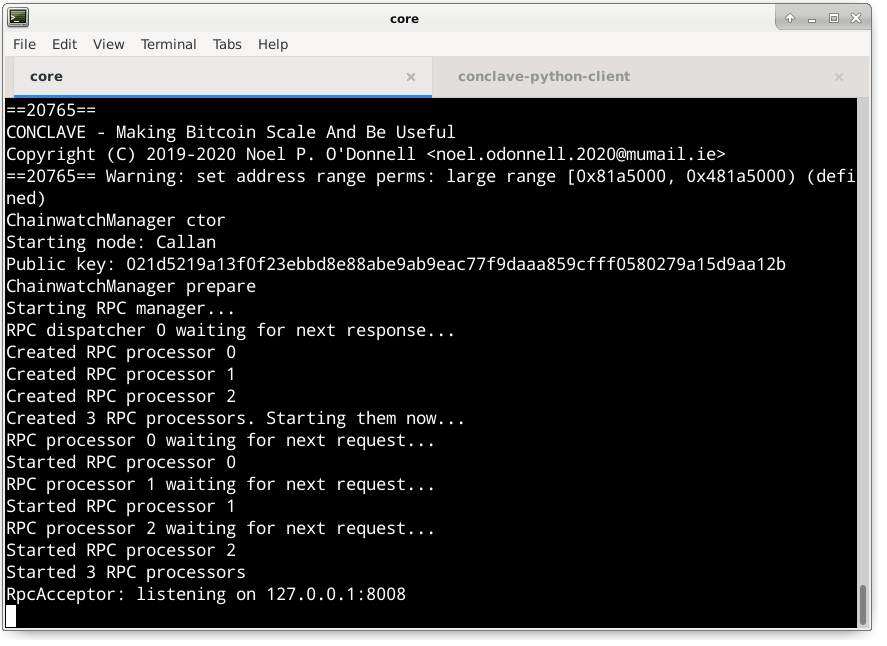
\includegraphics[width=200pt]{img/screenshot-1.png}
		  \captionof{figure}{\texttt{conclaved} after initial start-up}
		  \label{fig:test1}
		\end{minipage}%
		\begin{minipage}{.5\textwidth}
		  \centering
		  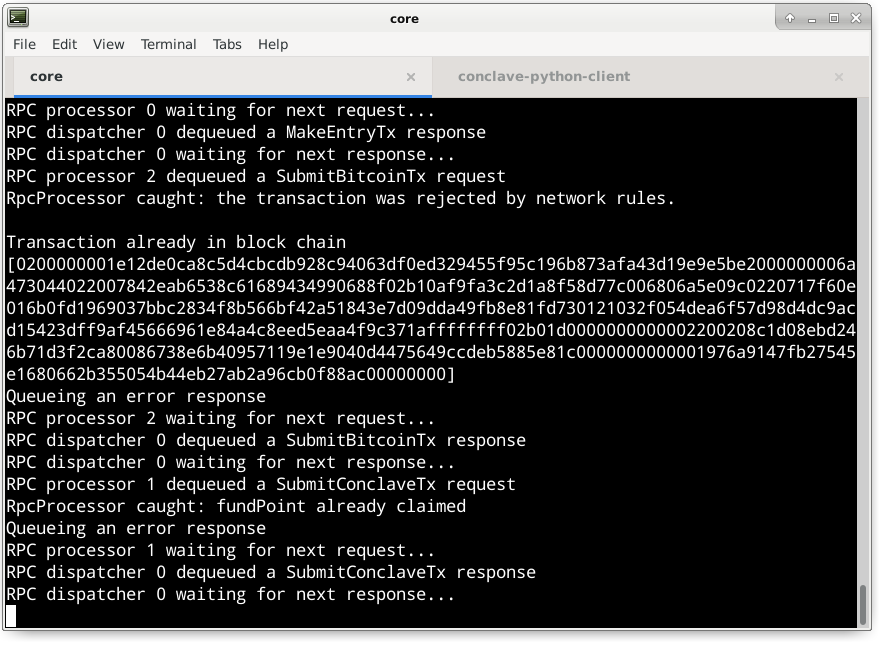
\includegraphics[width=200pt]{img/screenshot-2.png}
		  \captionof{figure}{\texttt{conclaved} after receiving transactions}
		  \label{fig:test2}
		\end{minipage}
		\break
		\begin{minipage}{.5\textwidth}
		  \centering
		  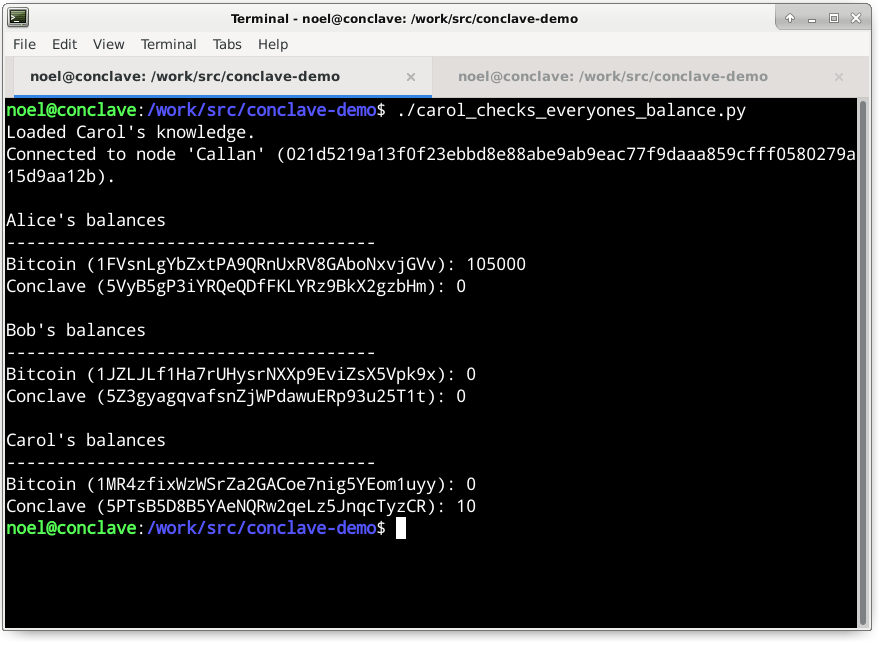
\includegraphics[width=200pt]{img/screenshot-3.png}
		  \captionof{figure}{Demo: Carol checks balances}
		  \label{fig:test1}
		\end{minipage}%
		\begin{minipage}{.5\textwidth}
		  \centering
		  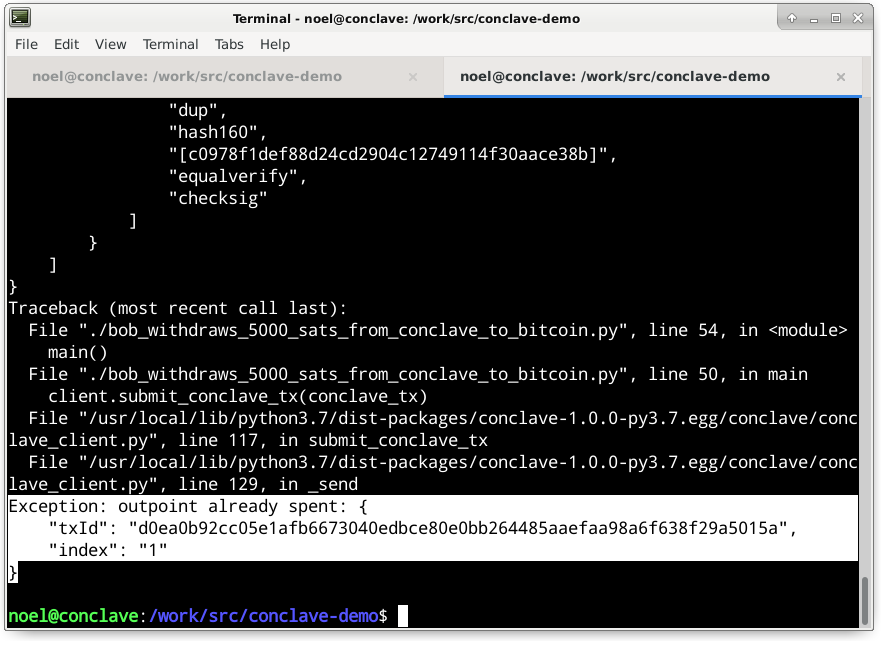
\includegraphics[width=200pt]{img/screenshot-4.png}
		  \captionof{figure}{Demo: Bob withdraws 5,000s, but output already spent}
		  \label{fig:test2}
		\end{minipage}
		\end{figure}
  \clearpage
  \chapter{Code Developed For This Project}
  The project consists of two codebases – the main C++ \index{C++} dæmon, and the python client. I also began work on Java \index{Java} and Javascript \index{Javascript} clients, however they are not part of the FYP deliverables. The demo is part of the python client codebase and can be found in the \textit{demo}  folder. All codebases live on Github \index{Github} under a project named \textit{conclave-network}. I’ve also mirrored them on the university’s Gitlab \index{Gitlab} system.
  \subsubsection{Conclave Core (C++)}
    \begin{tabular}{p{5cm}p{10cm}}
      Github: & https://github.com/conclave-network/conclave \\
      Gitlab: & https://gitlab.cs.nuim.ie/*******/conclave-core-2 \\
      Gitlab (original codebase): & https://gitlab.cs.nuim.ie/*******/conclave-core \\
    \end{tabular}
  \subsubsection{Conclave Client (Python)}
    \begin{tabular}{p{5cm}p{10cm}}
      Github: & https://github.com/conclave-network/conclave-python-client \\
      Gitlab: & https://gitlab.cs.nuim.ie/*******/conclave-python-client \\\
    \end{tabular}
  \clearpage
\end{appendices}
\printindex{}
\end{document}
